% \documentclass[letterpaper, twocolumn]{article}
\documentclass[sigconf]{acmart}


\usepackage{algorithm}
\usepackage{algpseudocode}
\usepackage{graphicx} 	% 1
\usepackage{wrapfig}
\usepackage{float} 		% to force figure placement
\usepackage{caption}
\usepackage{subcaption} % for the subfigure
\usepackage{amsmath} 	% to use \text{} command in math environment instead of \textrm{}
\usepackage{xcolor}
\usepackage{soul}       % for highlighting
\usepackage{xspace}
\usepackage{siunitx}
\usepackage[inline]{enumitem}
\usepackage{tikz}
\usepackage{enumitem}
%%%% Control the packages behavior
%\graphicspath{{../figures/}}

%\usepackage{booktabs} % For formal tables
%\usepackage{amsmath}
%\usepackage{hyperref}
%\usepackage{amssymb}
%\usepackage{tikz}
%\usepackage{pgfplots}
%\usepackage{lipsum}
%\usepackage{siunitx}
%\usepackage{subfig}
%\usepackage{flushend}
%\usepackage{libertine}
%\setlist{itemjoin ={,\enspace},itemjoin* = { and\enspace}}


%% New command for TODOs
\algnewcommand{\LeftComment}[1]{\Statex \(\triangleright\) #1}
\newcommand{\todo}[1]{}
\renewcommand{\todo}[1]{{\color{red} [{#1}]}}
\newcommand{\checkit}[1]{\textcolor{red}{Check---} \hl{#1}} 
\DeclareRobustCommand*\circled[1]{\tikz[baseline=(char.base)]{
            \node[shape=circle,draw,inner sep=1pt] (char) {#1};}}
\newcommand{\cis}{CIS\xspace}
\newcommand{\fullcis}{Coalesced Intermittent Sensor\xspace}
%\newcommand{\fullsys}{\sys: Battery-less Distributed Microphone}
%\newcommand{\fullsys}{Distributed Batteryless Intermittent Sensors}
%\newcommand{\fullsys}{Distributed Intermittent Systems: Theory and Practice}
\newcommand{\cim}{CICR\xspace}
\newcommand{\fullcim}{coalesced intermittent command recognizer\xspace}
\newcommand{\fullCIM}{Coalesced Intermittent Command Recognizer\xspace}
\begin{document}

% \title{\hl{Smart Fabric:} Continuous Sensing on Intermittent Power} 
\title{Continuous Sensing on Intermittent Power}

%\affiliation{\institution{Delft University of Technology}}
%\email{a.y.majid@tudelft.nl}
%
%\author{Patrick Schilder}
%\affiliation{\institution{Delft University of Technology}}
%\email{PATRIC@student.tudelft.nl}
%
%\author{Przemys{\l}aw Pawe{\l}czak}
%\affiliation{\institution{Delft University of Technology}}
%\email{p.pawelczak@tudelft.nl}
%
%\renewcommand{\shortauthors}{A.Y. Majid et al.}

%for single author (just remove % characters)
% \author{
% {\rm Amjad Yousef Majid}\\
% Delft University of Technology
% \and
% {\rm Patrick Schilder}\\
% Delft University of Technology
% % copy the following lines to add more authors
% \and
% {\rm Koen Langendoen}\\
% Delft University of Technology
% } 

\author{Amjad Yousef Majid}
\email{a.y.majid@tudelft.nl}
% \orcid{1234-5678-9012}
\affiliation{%
  \institution{Delft University of Technology}
}
\author{Patrick Schilder}
\email{p.t.schilder@student.tudelft.nl}
\affiliation{%
  \institution{Delft University of Technology}
}
\author{Koen Langendoen}
\email{k.g.langendoen@tudelft.nl}
% \orcid{1234-5678-9012}
\affiliation{%
  \institution{Delft University of Technology}
}
% \author{Stephan Wong}
% \email{j.s.s.m.wong@tudelft.nl}
% % \orcid{1234-5678-9012}
% \affiliation{%
%   \institution{Delft University of Technology}
% }

\renewcommand{\shortauthors}{A. Majid et al.}

%\keywords{}

\begin{abstract}
The main obstacles to achieve truly ubiquitous sensing are (i) the limitations of battery technology - batteries are short-lived, hazardous, bulky, and costly - and (ii) the unpredictability of ambient power. The latter causes sensors to operate intermittently, violating the availability requirements of many real-world applications. 
%
In this paper, we present the \textit{\fullcis} (\cis), an
intermittently-powered ``sensor'' that senses continuously! Although
a single node will frequently be off charging, a group of nodes can
--in principle-- sense 24/7 provided that their awake times are spread
apart. As communication is too expensive, we rely on inherent component
variations that induce small differences in power cycles. This basic
assumption has been verified through measurements of different nodes
and power sources. However, desynchronizing nodes is not enough.
%
An important finding is that a \cis designed for certain (minimal)
energy conditions will become synchronized when the available energy
exceeds the design point. Nodes employing a sleep mode (to extend
their availability) do wake up collectively at some event, process it,
and return to charging as the remaining energy is typically too low to
handle another event. This results in multiple responses (bad)
and missing subsequent events (worse) due to the synchronized charging.
To counter this undesired behavior we designed an algorithm to estimate the number of active neighbors and respond proportionally to an event. 
We show that when intermittent nodes randomize their responses to events, in favorable energy conditions, the \cis reduces the duplicated captured events by 50\% and increases the percentage of capturing entire bursts above 85\%. 


% The main obstacles to achieve truly ubiquitous sensing are (i) the limitations of battery technology - batteries are short-lived, hazardous, bulky, and costly - and (ii) the unpredictability of ambient power. The latter causes sensors to operate intermittently, violating the availability requirements of many real-world applications. 
% 
% In this paper, we present the \textit{\fullcis} (\cis), an intermittently powered ``sensor'' that senses continuously!
% Our key observation being that, the power cycles of energy-harvesting battery-less devices do not show correlation even when they are drawing energy from the same source, running the same application, and in close proximity.
% We challenged our observation using different real hardware and energy sources and showed that this observation holds.
% 
% Another important finding is that a \cis designed for certain (minimal) energy conditions requires no explicit spreading of awake times due to embedded randomness in the powering subsystem. However, when the available energy exceeds the design point, nodes employing a sleep mode (to extend their availability) do wake up collectively at the next event. This synchronization leads to problems as multiple responses will be generated, and -worse- subsequent events will be missed as nodes will now recharge at the same time.
% To counter this unwanted behavior we designed an algorithm to estimate the number of active neighbors and respond proportionally to an event. 
% We show that when intermittent nodes randomize their responses to events, in favorable energy conditions, the \cis reduces the duplicated captured events by 50\% and increases the percentage of capturing entire bursts above 85\%. 

\end{abstract}

\begin{CCSXML}
<ccs2012>
<concept>
<concept_id>10003120.10003138.10011767</concept_id>
<concept_desc>Human-centered computing~Empirical studies in ubiquitous and mobile computing</concept_desc>
<concept_significance>300</concept_significance>
</concept>
</ccs2012>
\end{CCSXML}

\ccsdesc[300]{Human-centered computing~Empirical studies in ubiquitous and mobile computing}
\keywords{Embedded systems, Energy harvesting, Ubiquitous computing, Intermittent Systems}

\maketitle


\section{Introduction}
\label{sec:introduction}

\begin{figure}
	\centering
	\begin{subfigure}{\columnwidth}
		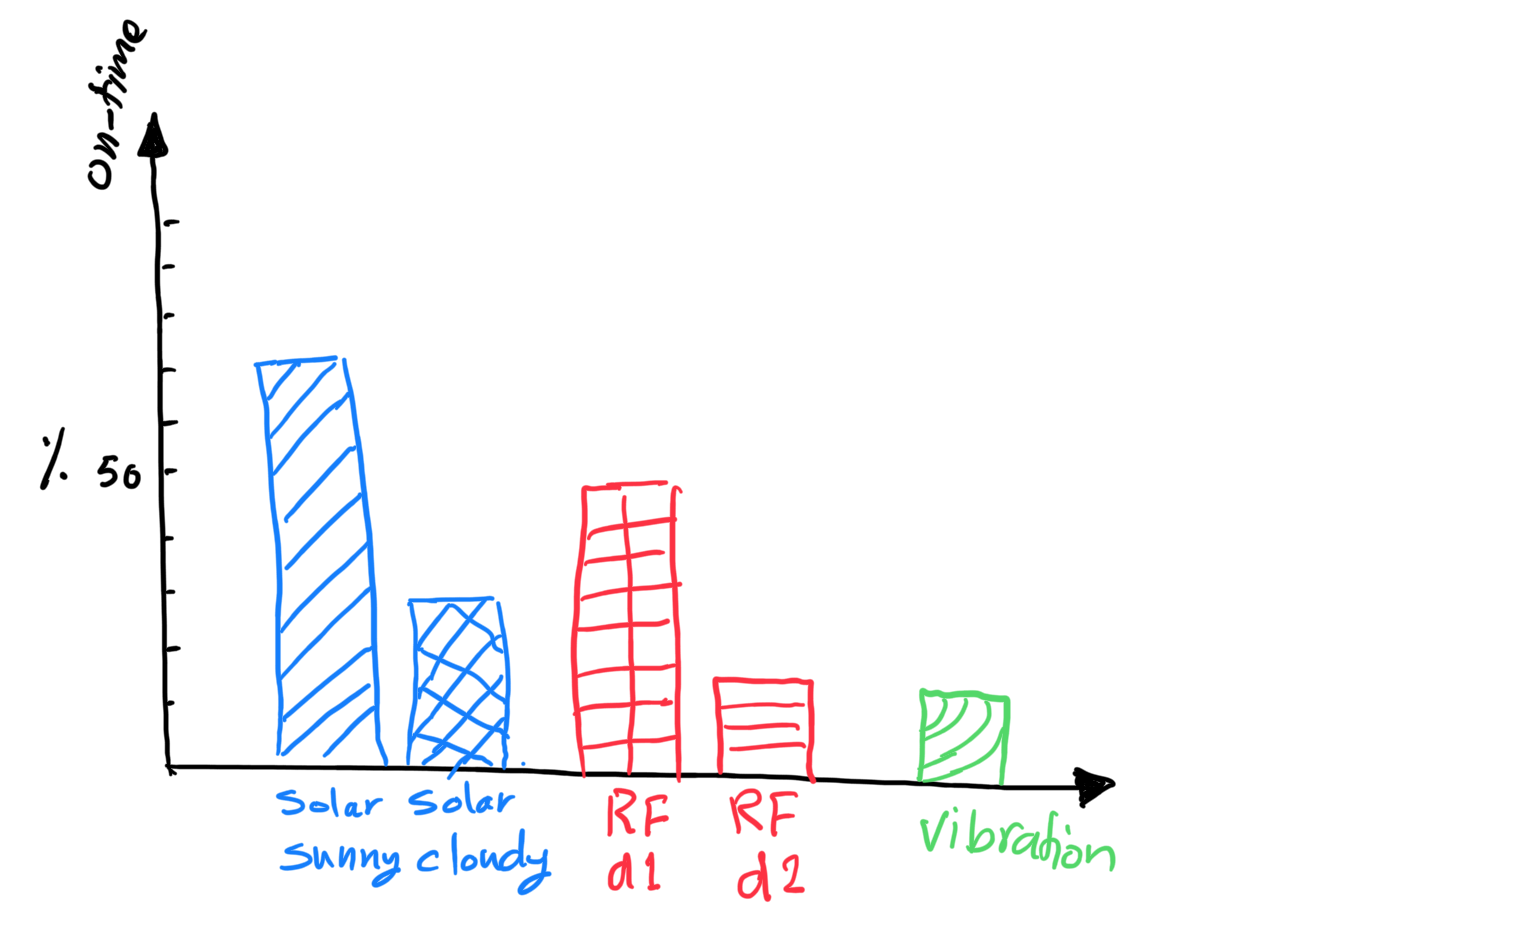
\includegraphics[width=\columnwidth]{figures/intermittent_problem}
		\caption{The on-time percentage of an intermittent device powered by different energy sources relative to its on/off cycle length}
		\label{fig:disInterSys}
	\end{subfigure}
	\begin{subfigure}{\columnwidth}
		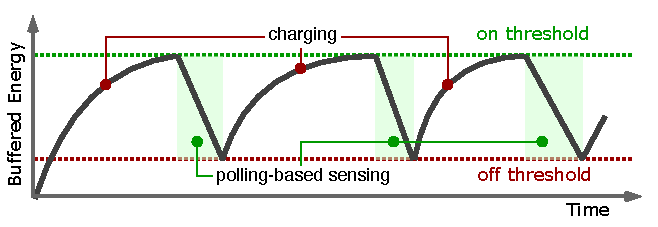
\includegraphics[width=\columnwidth]{figures/PowerCycleIntermittentSystem}
		\caption{The power cycle of an intermittently powered device.}
		\label{fig:powerCycle}
	\end{subfigure}
\end{figure}
%Intermittent software enables energy harvesting devices to run reliably despite arbitrarily timed power failures.  However, intermittent devices failed to  
%
%Self-powered tiny devices promise humanity with intelligent objects. Low cost, small size, and long operational time enable them to fundamentally change healthcare~\cite{ChenG.ISSCC2011}, water infrastructure~\cite{stoianov2007pipenet}, smart building~\cite{ardakanian2016buildsys,debruin2013monjolo}, and human-natural interaction~\cite{debruin2013monjolo}. \\
%%
%They operate by harvesting energy from ambient sources such as light~\cite{margolies_tosn_2016,margolies_infocom_2016}, vibration~\cite{gorlatova_sigmetrics_2014}, and radio frequency~\cite{rf_powered_computing_gollakota_2014} and able to compute, sense, actuate, and communicate~\cite{moo, naderiparizi_rfid_2015,flickersensys2017,smith_ubicomp_2006}.Ambient power, however, is marginal and unpredictable. Therefore,
%the execution is intermittent: it is triggered when a threshold amount of energy is buffered and terminated when the energy buffer is depleted. 

%%% Background, known information 

%An intermittently powered device (or node) starts by harvesting ambient energy. Once the harvested energy reaches a threshold, software execution begins and the energy in the buffer depletes gradually until the device shutdowns. This power cycle repeats indefinitely (Figure\,\ref{fig:powerCycle}). 

Intermittently powered devices use their environment as an energy source instead of batteries. Therefore, they promise small, cheap, and maintenance-free version of the current Internet of Things (IoT) edge devices. Driven by this vision, recent years have paid significant attention to intermittent systems~\cite{hicks2017clank,lucia2017intermittent,colin2016chain,colin2018termination,yildirim2018ink}. 
%
%%% knowledge gap, unknown information
However, their inherent sporadic operation patterns (Figure~\ref{fig:disInterSys}) have prevented researchers from demonstrating a real word applications, for example, \cite{colin2016chain,hester2017timely} present activity recognition applications without driving a real sensor to capture external signals.

%
%%% Hypothesis, question, purpose statement
This paper responds to the challenge of intermittent power supply by introducing the concept of \textit{distributed intermittent systems}. A distributed intermittent system is defined as the abstraction of a group of tiny intermittently powered devices (or nodes). The on-time of the distributed intermittent system should approach continuous time as the number of intermittent devices increases. However, the on-time and off-time of  distributed intermittent systems depend on the environment and the load. As such, we do not expect, for example, a linear relationship between the number of nodes and the overall on-time.

Controlling the on/off cycle of intermittent devices enables adapting them to many real world applications. For example, once a certain on/off cycle is preserved, an intermittent wake-up receiver can be implemented; intermittent acoustic monitoring system for monitoring engines modules---the sound produced by a deformed gear tooth---can be made. Moreover, with the advances in passive communication (such as passive light~\cite{}, and backscatter tag-to-tag~\cite{} communication) battery-free miniaturized sensors can form self-powered wireless sensor network to, for instance, create smart wallpaper and revolutionize smart buildings. 


This paper pushes the boundaries of intermittent systems by:
\todo{update the contributions and challenges}
\begin{itemize}
		\item introducing \textit{distributed intermittent systems} to control the duration of the up time of intermittent sensors and increase their responsiveness,
		\item investigating the relation between distributed intermittent systems power cycle and their environment,
		\item demonstrating the \textit{world first} distributed intermittent system: a distributed microphone. 
\end{itemize}
%\todo{add the challenges and contributions}
%%% Approach, plan of attack, proposed solution





% \section{Context Assumptions}
% \label{sec:background}
% Here a minimal amount of background information is presented to facilitate clarifying the technical sections of the paper. 

\subsection{Energy-harvesting Devices}

%1. why \textit{small form factors EH sensor nodes}\\
Small sensors are less intrusive devices, and therefore, many applications prefer them on the bigger ones 
% (imagine the difference in the implications of embedding a sensor of the size of 2 AAA batteries and a sensor of a few cubic millimeters in volume in a shoe for step counting).  
%
Long sensors lifetime is also desirable. However, long sensors lifetime and small form factors are conflict goals.
% 2. classify EH with continuous power and tiny EH with intermittent power \\
For example, rechargeable batteries paired with energy harvesters can continuously power sensor nodes for relatively long time. But, rechargeable batteries inherent normal batteries drawbacks including increasing the size and limiting the sensor lifetime (although much longer) as rechargeable batteries typically wear out after a few hundreds charging cycles~\cite{}.
%
However, if an application's requirements put hard constraints on the size of the sensors, then removing the batteries is one of the first options to be considered. 
Battery-less energy-harvesting sensors operate intermittently. They charge a small capacitor to ensure uninterrupted operations for a minimum certain duration. Once, the capacitor has been depleted, the sensor powers down, letting the energy-harvester to accumulate energy again. 
%
Intermittent operation raises many challenges such as how to enable applications to span their execution over power failure~\cite{}, and how to enable timeliness operations when the durations of the device power-downs are indeterminate~\cite{}.
%
Big capacitors may allow longer operational periods of time, but they also need more time to charge. 
In order for a capacitor to charge, the input voltage must be higher than the accumulated voltage in the capacitor. 
This phenomena makes charging big capacitors using tiny energy harvester less efficient~\cite{}. 
boosting ambient energy using an energy-conditioning circuit is possible on the expense of device complexity, form factor, energy consumption, and cost. 

\subsection {Speech types}
%
Speech recognition algorithms can be classified based on the type of speech that they can recognize into \textit{spontaneous speech, continuous speech, connected word,} and \textit{isolated word}~\cite{gaikwad2010review}.
Systems with \textit{continuous} or \textit{spontaneous speech} recognition are the closest to natural speech, but are the most difficult to create because they need special methods to detect words boundaries~\cite{gaikwad2010review}. This is less the case for the \textit{connected word} type, where a minimum pause between the words is required.
 The type with the least complexity is the \textit{isolated word} type. It requires a period of silence on both sides of a spoken word and accepts only single words. 
 
Voice is a natural way for the human to interact with small devices. However,
implementing speech recognition on resources---memory, computation power, and energy---limited platforms is challenging, to say the least. Therefore, we attempt to recognize, with our command recognizer prototype, the simplest type of speech, isolated words. 

\section{Related Work} % and Background}
\label{sec:relatedwork}
Recent advances in ultra-low-power microcontrollers along with the development of energy harvesters have enabled the creation of stand-alone battery-free sensors. These sensors operate intermittently because the power that they harvest is
weak and volatile.

\subsection{Energy-harvesting systems}
Energy harvesters have the potential to power devices indefinitely as they collect energy from perpetual energy sources. Sunlight, vibration, and radio frequency (RF) waves are examples of such energy sources. The power harvested from these sources vary wildly, for example, RF harvestable power ranges from
\si{\nano\watt}-scale when harvested from ambient signals to \si{\uW}-scale when collected from a dedicated RF signal emitter, and solar power varies from tens of \si{\uW} to tens of \si{\mW} when it is harvested by a solar panel of a few \si{\cm^2} illumination surface~\cite{lucia2017intermittent,rao2017ambient}.

Many battery-less energy-harvesting platforms have been proposed. Some of them
rely on dedicated external energy sources such as WISP -and its variants-, a
general wireless sensing and identification
platform~\cite{smith2006wirelessly,zhao2015nfc,zhang2011moo}; WISPcam,  an
RF-powered camera~\cite{naderiparizi2015wispcam} and, the battery-free
cellphone~\cite{talla2017battery}. Others, harvest from ambient sources such as
the ambient backscatter tag~\cite{liu2013ambient}, and the solar-powered
tag~\cite{majid2019multi}. Platforms that facilitate the development of
battery-less energy-harvesting systems have also been proposed. For instance,
Flicker~\cite{hester2017flicker}, a prototyping platform for battery-less devices; EDB~\cite{colin2016energy} an energy-interference-free debugger for intermittent devices;  and Capybara~\cite{colin2018reconfigurable}, a re-configurable energy storage architecture for energy-harvesting devices.

However, \emph{there is no energy-harvesting platform that considers the abstraction of many intermittent sensors (or nodes) and exploits the statistical energy harvesting differences between them to provide reliable sensing}.
% The paper is the first that considers the abstraction of a group of intermittent nodes and investigates the emerging collective duty cycle of the system. 
%experience. 

\subsection{Intermittent execution}
% What is the problem that requires intermittent execution
Intermittent execution models enable applications to progress despite frequent
power failures~\cite{van2016intermittent,colin2016chain,lucia2015simpler,bhatti2017harvos,gobieski2019intelligence}. To this end, they decompose an application into several small pieces and save the state of the computation on the transitions between these code segments. Therefore, intermittent applications do not return to the beginning of the program (i.e., \texttt{main()}) after each power failure.
%(in contrast to  applications that assume continuous power).
Instead, they resume execution from the last successfully saved progress state.   

% Sleep not to die 
% Intermittent systems are regarded as the successor of energy-aware systems. Dewdrop~\cite{buettner2011dewdrop} is an energy-aware runtime for (Computational) RFIDs such as WISP. Before executing a task, it goes into low-power mode until sufficient energy is accumulated. QuarkOS~\cite{zhang2013quarkos} divides the given task (i.e., sending a message) into small segments and sleeps after finishing a segment for energy recharge. However, these systems are not power disruption tolerant. In other words, if a system could not sustain the energy consumption of low-power mode and powers down, then all the computation progress will be lost. 

% checkpointing 
Mementos~\cite{ransford2011mementos} proposed a volatile memory \emph{checkpoint-based} approach to enable long-running applications on intermittently powered devices. DINO~\cite{dino} enables safe non-volatile memory access despite power failures. Chain~\cite{colin2016chain} minimizes the amount of data needed to be protected by introducing the concepts of \emph{atomic tasks and data-channels}. Hibernus~\cite{balsamo2014hibernus,balsamo2016hibernus++} measures the voltage level in the energy buffer to reduce the number of checkpoints per power cycle. Ratchet~\cite{van2016intermittent} uses compiler analysis to eliminate the need for programmer intervention or hardware support. HarvOS~\cite{bhatti2017harvos} uses both compiler and hardware support to optimize checkpoint placement and energy consumption. Mayfly~\cite{hester2017timely} enables time-aware intermittent computing. InK~\cite{yildirim2018ink} introduces event-driven intermittent execution.  
\emph{For our prototype implementation we adopt a power failure protection approach similar to that of DINO~\cite{dino}, see Section~\ref{sec:software}.}


\subsection{Speech recognition}
%  Speech recognition consists of several steps. The basic steps are:
% \textit{Speech recording and signal digitization}---a microphone records the sound waves and an ADC converts the microphone signal into a digital signal. A sampling rate of about 8 kHz is required to capture the frequencies of a human voice (100-4000Hz \cite{Bernal-Ruiz2005MicrocontrollerSystems}). \textit{Framing}---after that the digitized signal is divided into blocks of usually 10-30 ms~\cite{gaikwad2010review,delaney2002low,delaney2005energy} called frames. \textit{Features extraction}---for each frame a feature vector is extracted containing all the relevant acoustic information. \textit{Feature matching}---finally the extracted features are matched against features known to the recognizer. 

The speech recognition problem has been tackled from many angles and has experienced many breakthroughs. For example, the dynamic time warping (DTW) algorithm enables matching voice signals with different speed (or time) \cite{vintsyuk1968speech}. 
Approaches based on Hidden Markov Models showed much better performance than DTW-based ones~\cite{jelinek1997statistical}. Hence, they became the standard techniques for general-purpose speech recognition until artificial intelligent algorithms~\cite{hinton2012deep} outperform them. 
% Furthermore, many specialized hardware architectures for speech recognition have been proposed to, for instance, reduce energy consumption \cite{price2018low,price20156}. 

% The evolvement of the speech recognition algorithms has enabled them to recognize more complicated type of speech. 
% From a recognition algorithm perspective the speech can be classified
% Speech recognition algorithms can be classified based on the type of speech that they can recognize 
From a recognition complexity standpoint, we can classify the speech into \textit{spontaneous speech, continuous speech, connected word,} and \textit{isolated word}~\cite{gaikwad2010review}.
The \textit{continuous} and \textit{spontaneous speech} are the closest to natural speech, but they are the most difficult to recognize because they need special methods to detect words boundaries~\cite{gaikwad2010review}. This is less the case for the \textit{connected word} type, where a minimum pause between the words is required. The type with the least complexity is the \textit{isolated word}, as it requires a period of silence on both sides of a spoken word. 
 
% Voice is a natural way for the human to interact with small devices. However, 
Speech recognition on resources---memory, computation power, and energy---limited platforms is challenging, to say the least. Therefore, \emph{our command recognizer targets isolated-word type of speech}. 





















\section{Coalesced Intermittent Sensor}
\label{sec:coalInterSen}
The \fullcis (\cis) is the abstraction of a group of energy-harvesting battery-less sensor nodes seeking to approximate the continuous sensing availability characteristic of a battery-powered sensor. The design of a \cis needs to consider four main aspects: 
\begin{enumerate*}[label=(\roman*)]
\item how the nodes' awake time is distributed; 
\item the consequence of emulating continuous sensing availability by chaining multiple short on-times; 
\item the effect of the environment on the \cis's availability; and 
\item the spacial coverage of the event of interest, which determines the diameter of the \cis.
\end{enumerate*}

However, let us first characterize the power cycle of an energy-harvesting battery-less device. 
An energy-harvesting intermittent node frequently switches between off and on, charging energy and operating. We can characterize, from a time perspective, this charge-discharge (or power) cycle using the following notation, ($t_\text{on}$, $t_\text{p}$), where $t_\text{on}$ is the node's uptime interval, and $t_\text{p} \coloneqq t_\text{on} + t_\text{off}$, where $t_\text{off}$ is the node's charging time interval.

\subsection{Sensing}
The ability of a \cis to sense depends on the availability of its intermittent nodes and on the characteristics of the event of interest. 

\subsubsection{Coalesced availability}
\label{subSec:availability}
The \cis's availability is the projection of its underlying intermittent nodes' on-times on the time axis. 
To determine the expected availability of a \cis, the strategy being employed to distribute its nodes' on-times must be first specified.
%
\paragraph{Explicit on-time division strategy}
A \cis can build on top of the recent advancements in passive (light or RF)
communication~\cite{liu2013ambient}
%\cite{LuzLink}
and ultra-low-power timers~\cite{hester2017timely} to apply a
time-division multiplexing strategy, minimizing overlapping on-times. For
example, a node calculates its average on-time $\overline{t_\text{on}}$
and off-time $\overline{t_\text{off}}$ for a certain number of power
cycles. Then, it encodes the information $({\overline{t_\text{off}},
\overline{t_\text{on}}})$ in a message and broadcasts it to its neighbors at
the beginning of it's next power cycle.
When a node receives this message 
it can then adjust
its power cycle, relative to the transmitting node's cycle, by increasing
(or decreasing) its power consumption to shorten (or lengthen) its
on-time and subsequently shift its power cycle to a different time slot.

With such explicit on-times control strategy, a \cis of $N$ nodes with on-time of $\overline{t_\text{on}}$ and off-time of $\overline{t_\text{off}}$ will have an availability 
$= \min \left(N\times \frac{\overline{t_\text{on}}}{\overline{t_\text{p}}}, 100\%\right)$. However, we expect such an approach to introduce significant overhead as a scattering algorithm (e.g., \cite{giusti2007decentralized}) must be frequently executed, messages need to be exchanged, and clocks should be synchronized. Therefore, we propose a different on-times spreading strategy.  
%
\begin{figure}[t]
		\centering
		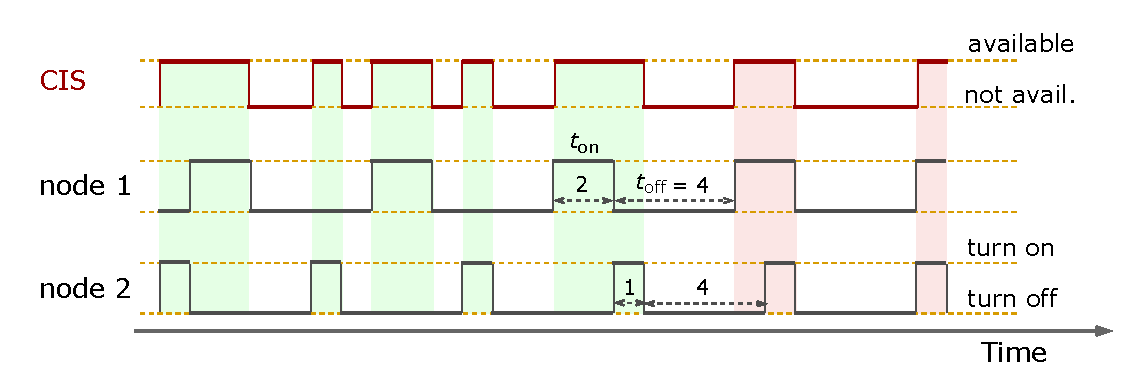
\includegraphics[width=\columnwidth]{figures/cisOntime}
		\caption{A \fullcis's availability is the emerging collective
		on-time of its intermittent nodes' on-times. The difference
		between the power cycles leads to a constant relative shift
		between the nodes' duty cycles. This, in turn, causes their on-times to be uniformly distributed on the overall power cycle. The red bars indicate a minimum \cis time span---\cis nodes are overlapping---whereas the green bars show the maximum time span of the \cis.}
		\label{fig:cisOntime}
\end{figure} 
%
\begin{figure}
		\centering
		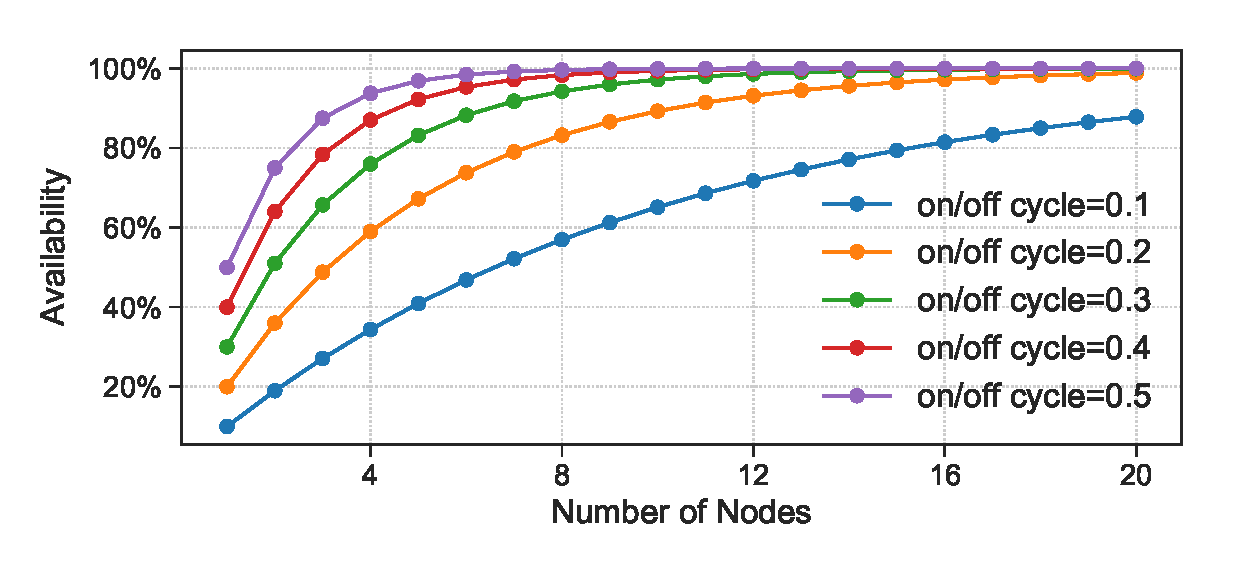
\includegraphics[width=\columnwidth]{figures/cisModel_2}
		\caption{\fullcis availability for a different number of nodes and different duty cycles. The nodes are uniformly distributed and the \cis on-time evolves, when adding new nodes, according to equation~\ref{eq:cisModel}.}
		\label{fig:cisModel}
\end{figure} 
%
\paragraph{Implicit on-time division strategy} 
With no information being exchanged between intermittent nodes, the best \cis can do is to uniformly distribute its node's on-times and maintaining this distribution over time. 
The key observation to approach uniform distribution is to ensure that the lengths of the node's power cycles are randomized, avoiding nodes being in lockstep indefinitely.

Let us start by assuming that we have a \cis of two nodes with idealized power cycles and these nodes have the same initial conditions. The availability of this \cis equals $t_\text{on}$ as the nodes are in perfect synchronization (the two nodes wake up and power down together). 
To extend the availability of this \cis, one of the node should
shift its on-time away from the other. If one of the nodes sleeps for $t$\,units of time, then the on-time of this power cycle will be $t_\text{on}+\Delta t$. Consequently, the length of this power cycle will be $t_\text{p} + \Delta t $, delaying the next awake time by $\Delta t$.
If the node sleeps only once, then availability of the \cis will equal $\min \left(2\times t_\text{on}| t_\text{on}+\Delta t\right)$

However, if the initial conditions are unknown, then shifting a node's on-time a constant number of times may cause the initially desynchronized nodes to become synchronized, collapsing the \cis's availability instead of extending it. Therefore, a safer option is to \emph{constantly} shift the awake time of the node. In this case, the on-time will shift over the entire power cycle of the other node, spending $\frac{ t_\text{off} }{t_\text{p}}$ and $\frac{ t_\text{on} }{t_\text{p}}$ of the time overlapping with the other node's off-time and on-time, respectively. This behavior is illustrated in Figure~\ref{fig:cisOntime}, where node 1 and node 2 have power cycles of (2,6) and (1,5). Following the time axis from the left to the right, we can observe that the position of the on-time of node 2 is shifted by -1 unit of time relative to the on-time of node 1 after each power cycle of node 1. This implies that the on-times of the two nodes are $\frac{1}{3}$ of the time cluster together and $\frac{2}{3}$ of the time they are apart (from an external event standpoint, the on-times are uniformly distributed over the longest power cycle, as they have the same probability to be anywhere when the event arrives). To model the availability of a \cis of $N$ nodes, we first model the nodes' on-times and power cycles.
%
If we represent the on-time of a node with a random variable $R_\text{n}$ and find its expected value $E(R_\text{n})$ then we can approximate \emph{any} \cis node's on-time with mean of the expected values of the nodes' on-times, i.e., $t_\text{on} = \frac{1}{N} \times \sum_{i=1}^{N} E(R_\text{n})^i$ (intuitively, since we are assume \cis nodes have the same energy buffer, then their expected on-times should approach the same value). Using a similar analogy, we can define the mean of the expected values of the power cycles lengths as $t_\text{p} = \frac{1}{N} \times \sum_{i=1}^{N} E(R_\text{p})^i$. Now, we can model the availability of a \cis of $N$ nodes as:
%
% If we extend the previous scenario to a \cis of $N$ nodes such that nodes' on-time $t_\text{on}$ is approximated with the mean of the expected values of
% \in \{ t_\text{on}^1,t_\text{on}^2,... t_\text{on}^N \}$ and their power cycles $t_\text{p}^i \in \{ t_\text{p}^1,t_\text{p}^2,\text{...} t_\text{p}^N \}$, then we can model the \cis availability as,
%	
\begin{equation}
	A_\text{v}(N) = A_\text{v}(N-1) + \left(1-A_\text{v}(N-1)\right) \times \frac{t_\text{on}}{t_\text{p}},
		\label{eq:cisModel}
\end{equation}
%
for the initial case where $N=1$ we define $A_\text{v}(0)\coloneqq 0$. Figure~\ref{fig:cisModel} shows the availability of \cis when $N\in\{1,2,..,20\}$ and nodes' duty cycles $\frac{t_\text{on}}{t_\text{p}}\in\{10\%,20\%,..,50\%\}$.
%
We can conclude from the above discussion that to approach uniform distribution of nodes' on-times, the lengths of the power cycles need to be randomized~\footnote{Note that, having power cycles of lengths that are multiples of each other is a very unlikely as nodes' energy buffers are assumed to be of the same size.}. 

The power cycles of energy-harvesting battery-less devices are inherently randomized and different because the power source (ambient energy) is volatile and the harvesters are not perfect devices (notice that, even battery-powered wireless sensor nodes require a synchronization protocol to correct for the drift in their local clocks). Our own measurements using different energy-harvesting devices and different energy sources, i.e., solar and RF, also confirm that the power cycles of intermittent nodes are different and randomized (Figure~\ref{fig:power_cycles}). Therefore, we expect their on-times to be uniformly distributed (we will challenge our expectation in Section~\ref{sec:evaluation}). 
%
\begin{figure}[t]
		\begin{subfigure}{.49\columnwidth}
			\centering
			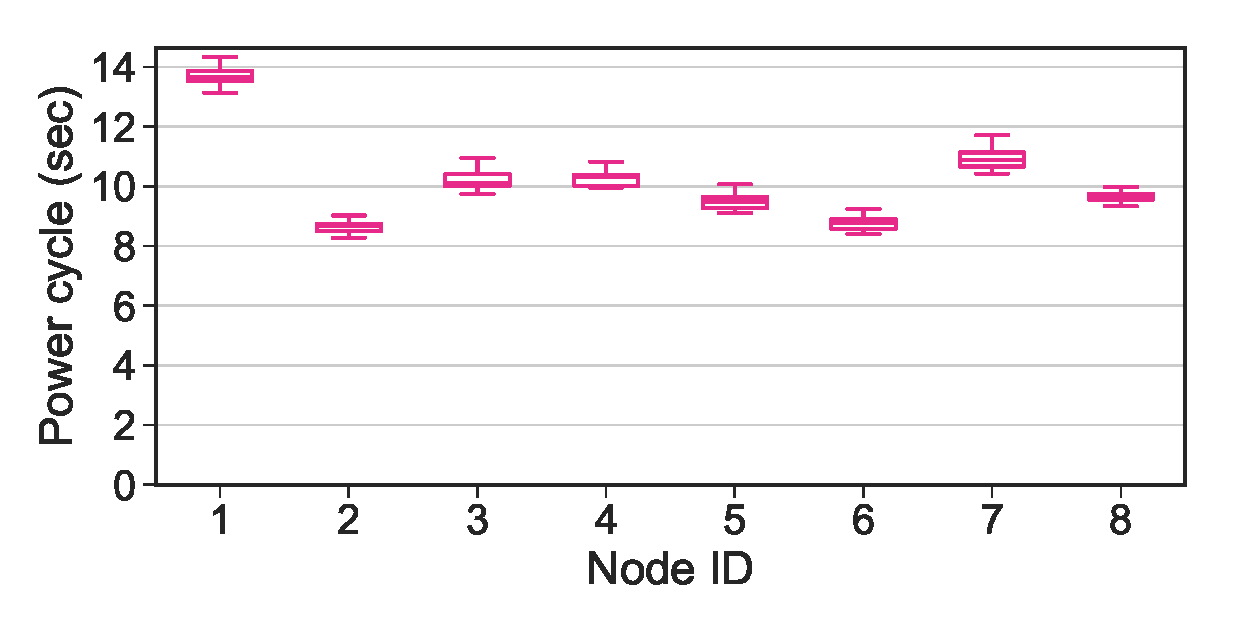
\includegraphics[width=\textwidth]{figures/light_power_cycles_len}
			\caption{Light ($680\si{\mu F}$) }
		\end{subfigure}\hfill
		\begin{subfigure}{.49\columnwidth}
			\centering
			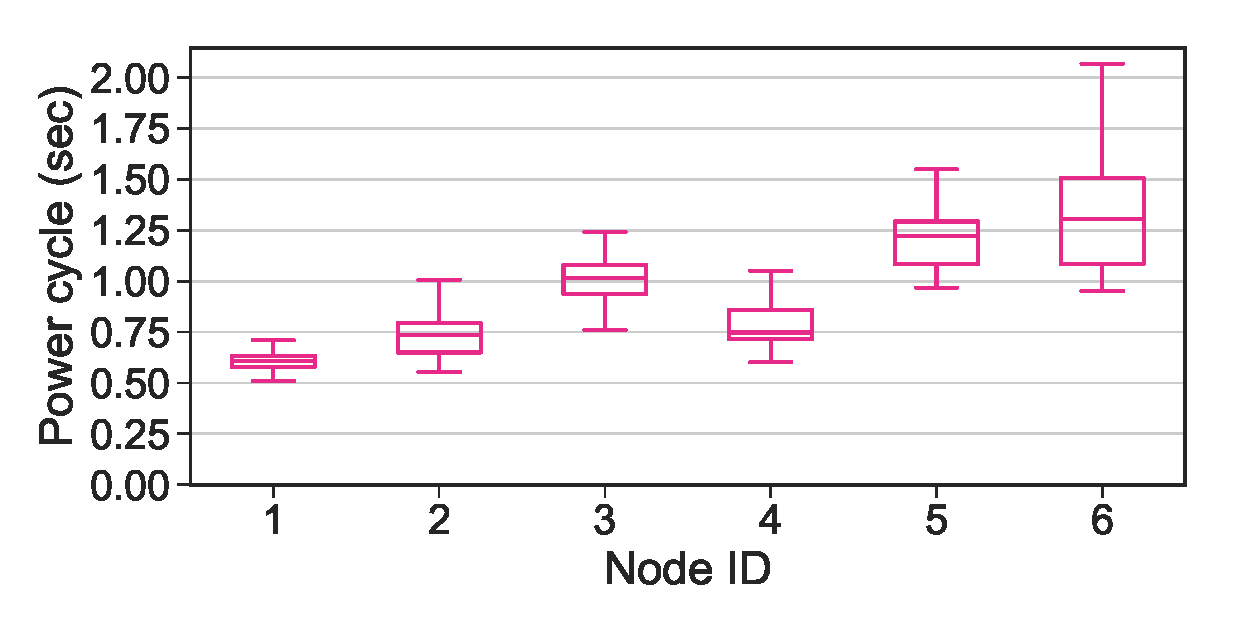
\includegraphics[width=\textwidth]{figures/rf_power_cycles_len}
			\caption{RF ($47\si{\mu F}$)}
		\end{subfigure}\hfill
		\caption{Nodes' power cycles length for different ambient energy sources, and different energy buffer sizes.}
		\label{fig:power_cycles}
\end{figure} 
%
\subsubsection{Events classification}
\label{sec:event_classification}
The availability of a \cis is not a single stretched interval: it is a chain of short intervals. Therefore, it is important to classify from a \cis perspective which types of events the \cis is best suited for. 
%
\begin{itemize}[leftmargin=*]
\item \textit{Short events}: are events that can be captured using single intermittent node. For example, a spoken word can be seen as a short event if the energy needed to record it is less than what the energy buffer, i.e., the capacitor, can store.
\item \textit{Long events}: are events that need more energy to be completely captured than what the energy buffer can store. Long events can be subdivided into three categories: 
	\begin{itemize}
		\item \textit{Simple}: is a long event that can be captured
		using single intermittent node---capturing part of it is
		sufficient to obtain all the information of interest---such as
		the sound produced by the friction between two moving parts of
		an engine.% (\textit{Why this is not a short event? keep reading}). 
		\item \textit{Burst}: is a group of short events that requires multiple intermittent nodes to be captured such as a command of a few words (e.g., room temperature up).
		\item \textit{Complex}: is a long event that must be fully captured to be recognized. For example, sampling a gyroscope attached to a moving device (e.g., a toothbrush).

	\end{itemize}
\end{itemize}
%
Based on the above classification, we can argue that designing a \cis for long events is not like designing it for capturing short ones. For example, while capturing a short event may require continuous \cis availability, capturing a long simple event that is longer than the power cycle $t_\text{p}$ does not require extending the availability of a single intermittent node. Furthermore, capturing a long complex event may require data fusion and processing that require the \cis{}s' nodes to communicate the raw data to a more powerful node, which may lead to significant overhead. However, this paper focuses on short and long bust events as they cover a wide range of applications (e.g., voice-controlled human-object interface). 
%ToDo what about the long simple event (it is a relax version of the problem of capturing short event, i.e., less less strict availability is required)

\subsubsection{Effective Availability}
%
\begin{figure}
		\centering
		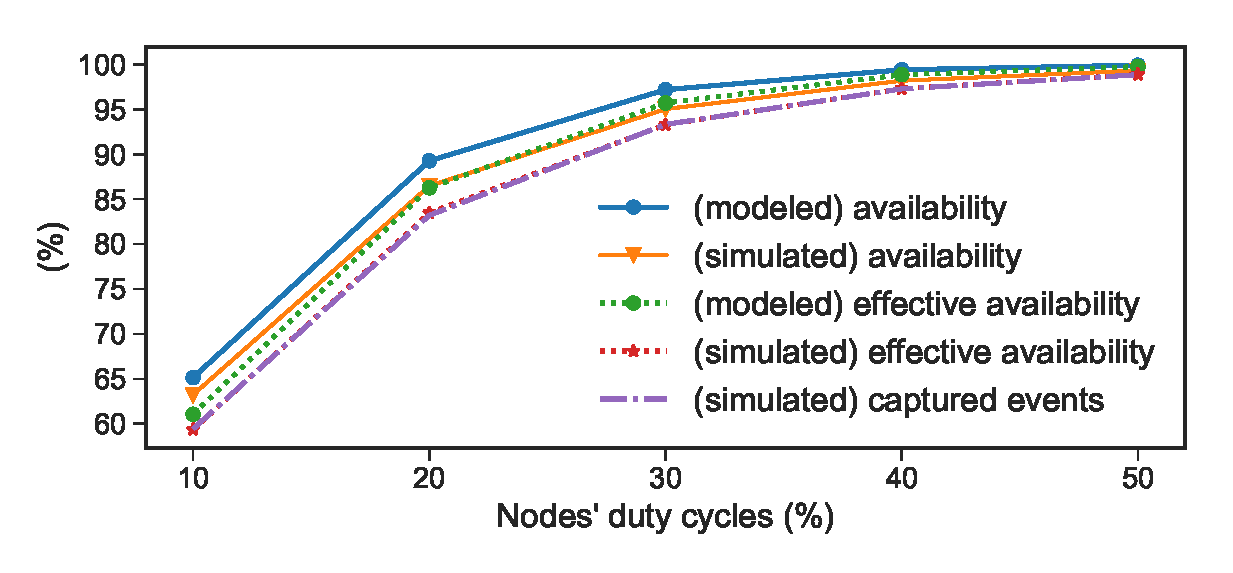
\includegraphics[width=\columnwidth]{figures/effective_availability_2}
		\caption{Simulating the availability, the effective availability, and successfully captured events of a \cis of 10 nodes with a node duty cycle $\in \{10\%, 20\%,...,50\%\}$.}
		\label{fig:cis_simulation}
\end{figure}
%
Approaching continuous availability does not mean that a \cis can successfully capture all events. It can happen that an event is being only partially captured by one or more nodes, which may lead to unsuccessful event detection. Therefore, it is important to specify the effective availability of a \cis that leads to a successful event capturing (which we assume leads to successful sensing). 

\paragraph{Polling-based Sensing}
Let us assume that we have a \cis of a single intermittent node monitoring a short event of length $t_\text{e}$. For capturing the entire event, the event has to arrive within the interval, $t_\text{on} - t_\text{e}$, which we call, the effective on-time of an intermittent node.
Therefore, the effective availability of a \cis of $N$ nodes is the joined effective on-times of the underlying intermittent nodes, which can be modeled as,
%
\begin{equation}
		A_\text{v}(N) = A_\text{v}(N-1) + \left(1-A_\text{v}(N-1)\right) \times \frac{t_\text{on} - t_\text{e}}{t_\text{p}},
		\label{eq:cisSenseModel}
\end{equation} 
%
\paragraph{Event-driven Sensing}
An intermittent sensor has a limited energy budget per power cycle. When it is tasked with a polling-based sensing activity, its energy consumption, generally, switches between two levels: zero when charging and maximum when sensing. However, in event-based sensing, a node puts its microcontroller into low-power mode and waits (or listens) for an external event to wake up the microcontroller. For example, in our prototype, a voice-controlled command recognizer, we exploit the microphone's wake-on-sound feature to send an interrupt to the microcontroller, which will then start recording the sound samples from the microphone. 
This wake-on-event style of operation is important as the minimal energy consumption during sleep significantly prolongs the period during which an event can be handled (for example, our prototype consumes 7 times less energy during sleep compared to being active).
To model the effective \cis availability when it is tasked with event-based sensing the change in energy consumption between the sleep and active mode must be taken into account. Since the event itself times when the node changes its energy consumption, we can model the effective availability as,
\begin{equation}
		A_\text{v}(N) = A_\text{v}(N-1) + \left(1-A_\text{v}(N-1)\right) \times \frac{t_\text{s} - (t_\text{e} \times\frac{p_\text{a}}{p_\text{s}}) }{t_\text{sp}},
		\label{eq:cisEventSenseModel}
\end{equation}
%
where $t_\text{s}$ is the expected sleep time of the \cis nodes, 
 $t_\text{sp} \coloneqq t_\text{s} + t_\text{off}$, 
 and $p_\text{a}$ and $p_\text{s}$ are the power consumption in active and sleeping mode, respectively.
 Notice that, there is a subtle point about equation~\ref{eq:cisEventSenseModel} as when an event arrives the node wakes up, consuming more energy. Therefore, its uptime shrinks. We, for simplicity, modeled this effect by extending the event time with the same factor. This is sufficient to say if that the event will be fully captured or not (effective availability).
%
\subsubsection{Simulation}
As a first sanity check on our models, we simulated $10^5$ power cycles of a \cis of 10 nodes (Figure~\ref{fig:cis_simulation}). The duty cycles of the nodes range from $10\%$ to $50\%$, while the event length is fixed at $3\%$ of the power cycle length, $t_\text{p}$. The on-times and event arrivals were uniformly distributed over the power cycles. 
The results clearly confirm our models and support our argument about the distinction between \cis's availability and effective availability (notice that the percentage of captured events matches the effective availability). 
The importance of this distinction---availability versus effective availability---is a function of the value $\frac{t_\text{e}}{t_\text{on}}$; observe the difference between availability and effective availability when nodes' duty cycle is $10\%$ (large effect) and $50\%$ (negligible effect).
%
%
\subsection{Environment}
Ambient energy controls the availability of a \cis nodes.  Consequently, it also controls their collective response to external events. When it rises, it extends nodes' on-times that may lead node's power cycles to be synchronized on the arrival of some external events, compromising the \cis's overall availability. To overcome this problem the \cis nodes must be power-state aware and able to estimate the number of active nodes in the \cis.
%
\subsubsection{Power States}
\label{sec:power_state}
A \cis can experience a wide range of ambient power intensities. For example, a solar-powered \cis may harvest no energy at night, modest energy from artificial light, and abundant energy from direct sunlight.  Generally, we can identify four different \cis powering states: 
\begin{itemize}[leftmargin=*]
	\item \textit{Targeted power state}---These are the powering conditions that a \cis is designed for. In these  conditions, the \cis should work intermittently and have sufficiently randomized power cycles to uniformly distribute its intermittent nodes on-times and meet the desired availability (Figure~\ref{fig:cisModel}). In general, the targeted powering conditions should be near worst energy harvesting conditions to ensure that the system is properly functioning for the majority of the time.
	\item \textit{Under-targeted power state}---Ultimately, the ambient energy is an uncontrollable power source, and it is not hard to imagine scenarios where a \cis will be under-powered or even comes to complete and long power down (for example, a solar \cis will come to a perpetual power down in darkness). In general, for under-targeted energy conditions, the \cis behavior can be considered as undefined.
%
\begin{figure}
	\centering
	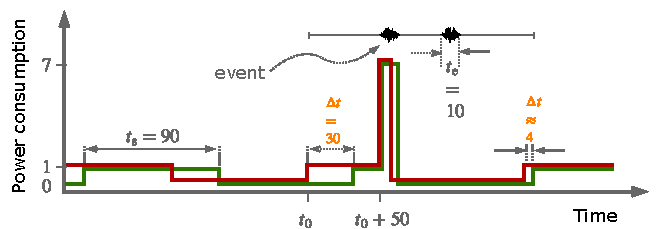
\includegraphics[width=\columnwidth]{figures/hibernatingState}
	\caption{
	Capturing events may lead synchronized power cycles of nodes that were
	in low-power mode. In particular, if some of the nodes power down while
	capturing an event, then this implies that these nodes slept (prior to
	the event) longer than the nodes that capture the event. This means
	that the nodes that have died spent their energy slower (they stayed
	longer in sleep mode); therefore,  their overall uptime is longer than
	the uptime of the node the captured the event. In other words, the
	nodes that woke up earlier have stayed longer on, and therefore, the
	next power cycles are more synchronized, see the $\Delta t$ before and after the event.
	% \fullcis is in a hibernating power state when the energy harvesting rate approximates the energy consumption rate at the sleeping (or low-power) mode. In this state, the intermittent nodes lose the randomization in their power cycles. Thus, all the nodes capture the same event and power down shortly after missing the subsequent ones. Consequently, the \cis senses intermittently and does not take advantage of its redundant intermittent nodes to approach continuous sensing.
	}
	\label{fig:noRand}
\end{figure} 
%
	\item \label{it:hibernating} \textit{Hibernating power state}---In event-driven sensing, nodes sleep in low-power mode waiting for an event to wake them up. This mode extends \cis nodes' on-times and makes them overlap significantly. Moreover, the on-times overlap even more, when ambient energy level rises (favorable energy conditions). If an event arrives in such conditions, it will wake up many nodes, causing them to consume their buffered energy much faster. Some of these nodes will power down before capturing the entire event, while others survive. This difference in how much energy is spent in active and sleep mode causes these nodes to tend to synchronize their power cycles after the event. To understand why
	% , you should realize that the nodes that capture the entire event have the shortest uptime as they stayed in active mode for the entire event duration; therefore, they consume their the fastest. 
	% The nodes that died while capturing the event must have been sleeping for a longer time than the node that capture the event. 
	%  for a longer uptime as they stayed only for a part of the event duration in the active mode, which implies that they stayed a number of time longer in sleep mode
	% The uptime of the surviving nodes, for the this power cycle, is the shortest as they stayed in active mode for the entire event. 
	% However, the nodes that died while capturing the event must have been sleeping for a \emph{longer} time than the node the captured the event. 
	% Therefore, the died-while-capturing nodes had gone into sleep mode \emph{before} the surviving nodes and their uptime is longer than the nodes that successfully captured the event. Therefore, the power cycles after the event tend to cluster together.
	% Since the energy buffers of the nodes are the same, the nodes' up-times that the event arrives in will be significantly different; nodes that die while capturing the event spend their energy budget slower as they spend less time in active mode than the nodes that capture the entire event, which, in turn, implies that the nodes that die while capturing the event must have been sleeping for a longer time than the nodes that capture the event. 
	%
	% If we assume that nodes have the same energy buffers, then the nodes that died before finishing the event should have been sleeping for a \emph{longer} time than the nodes the capture the entire event (because they slept for a long time, they could not finish capturing the event). However, nodes that captured the entire event have a \emph{shorter} overall uptime than the nodes the have died while capturing the event because they stayed \emph{longer} in the active mode (because they stayed longer in active mode, they consume their energy budget faster). This will lead the nodes' power cycles to tend to synchronized after the event. 
	%
	let us analyze the example presented in Figure~\ref{fig:noRand}. The figure shows the power traces of two nodes. the nodes consume 7 times more power in active than in sleep mode (our prototype has a similar power consumption ratio, Table~\ref{tab:power_usage}). Further, it shows that a node sustains the low-power mode for 90 units of time, $t_\text{s} = 90$; therefore, the maximum buffered energy can be calculated as 
	%
	$$E_\text{buf}=t_\text{s} \times p_\text{s},$$
	%
	where $p_\text{s}$ is a node's power consumption in sleep mode. If we focus on the power cycle with the first event, then we see that node $R$ powers up at $t_\text{0}$, and it remains in low-power mode for 50 units of time, whereas node $G$ spends only 20 units of time before the event arrives. Now, we can calculate when these two nodes will power down and compare the difference, $\Delta t$, before and after the event. A node will turn off when the buffered energy is depleted. This can be expressed as follows, 
	%
	$$
	E_\text{buf} = t_\text{se} \times p_\text{s} + t_\text{on} \times p_\text{a},
	$$
	%
	where $ t_\text{se}$ is the sleep time of the power cycle that an event arrives in, $t_\text{on}$ is a node's on-time and $p_\text{a}$ is the power consumption in active mode, which can be expressed as $p_\text{a}=\frac{\delta}{p_\text{s}}$. $ t_\text{se}$ and $ \delta$ are given and $p_\text{s}$ can be eliminated; thus to find when the nodes will power down we need to find $t_\text{on}$ for both nodes. By substituting the given values we find $t_\text{on}$ to be 10 and 5.7 units of time for the $G$ and $R$ node, respectively. Therefore, $\Delta t$ becomes 4.3 while it was 30 before the event (notice, $\frac{30}{7} \approx 4.3$). 
	%
	In general, nodes that die while capturing the event must have started their power cycles \emph{before} the nodes that capture the event.
	Further, the uptime of the died-while-capturing nodes is \emph{longer}
	than the nodes that capture the event because they spend less time in
	active mode. Therefore, the difference,  $\Delta t$, between the power
	cycles of a died-while-capturing node and a node the successfully
	captures the event becomes smaller. This difference shrinks by a factor
	$\delta = \frac{p_\text{a}}{p_\text{s}}$.
	When the events arrive in burst this becomes a significant problem, as a \cis will capture multiple copies of the first event, while missing the subsequent ones. 

	%TODO Connected with above text%
	% Consequently, the \cis may miss the next incoming events (specially if the events happens to arrive in bursts) causing it to sense intermittently instead of continuously (Figure~\ref{fig:hibernatingState}). 
	%
	\item \label{it:continuous} \textit{Continuous power state}---Under direct mid-noon sun a tiny solar panel may provide sufficient power to run a sensor node continuously. In such conditions, a \cis node will be available and able to sense continuously. Therefore, the job of a single node will be repeated $N$ times, and instead of sending a single message to a sink---to push the data to the Internet---$N$ identical messages will be sent.
	These messages will collide as they are sent at about the same time, causing the information to be lost; if they arrive, however, they -except the first one- will waste energy of the sink as they carry the same information.  
	 % at about the same time causing them to collide or waste energy as they replicated the same information that has been delivered by the first message. 
				
\end{itemize}
%
The inefficiencies highlighted in the hibernating and continuous power states can be mitigated by enforcing randomization on the response of intermittent nodes 
% (Figure~\ref{fig:rand})
: when a node is woken up by an external event it responds to that event with a certain probability. However, if the randomized response is enforced all the time, then the \cis will have a lower probability of catching events during the targeted energy conditions state. Therefore, the \cis has to distinguish between the targeted and above-targeted energy conditions and randomize its response only during the hibernating and continuous power states. 

Furthermore, responding with a constant probability during the above-targeted energy conditions is inefficient, as the number of active nodes is a function of the total number of intermittent nodes and the power intensity at that time. Therefore, efficient randomization requires intermittent nodes to estimate the number of active nodes and respond proportionally. Our proposed algorithm for estimating the number of active nodes depends on the nodes ability of measuring their on-times and off-times.

\subsubsection{Intermittent Timing}
\label{subsec:interTimer}
%
\begin{figure}[t]
		\centering
		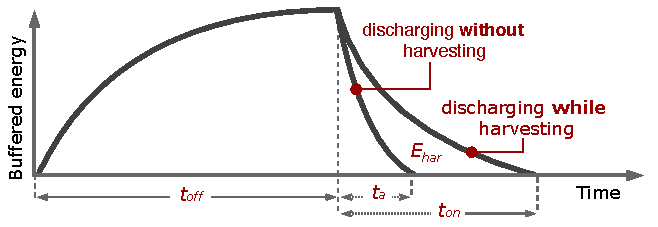
\includegraphics[width=\columnwidth]{figures/softwareClock}
		\caption{The difference in the time of discharging the energy buffer---a node's on-time---when an energy-harvesting device is allowed to charge while operating, and when it is not allowed.}
		\label{fig:softwareClock}
\end{figure} 
\begin{algorithm}[t]
	\captionof{algorithm}{off-time estimation}
    \label{algo:offTime}
    \small
    \begin{algorithmic}[1]
		\State $R_\text{cntr}\text{++}$   \Comment{reboot counter} \label{lin:i}
			% \State $i \leftarrow $ \Call{$f_\text{reboot}$}{$i$} \Comment{$i$ is a persistent variable} \label{lin:i}
		\State $E_\text{buf}$ \Comment{Size of energy buffer}
		\State $t_\text{a}$ \Comment{time of discharging $E_\text{buf}$ at load $a$, no harvesting}\label{lin:ta}
		\State$ X_\text{cy} $ \Comment{time every $X$ power cycles} 
		\LeftComment{\colorbox{lightgray}{Code executed on each $X$ power cycles \hspace{3cm} }}
		\If{$(R_\text{cntr} == X_\text{cy})$}
			\State \Call{$f_\text{load}$}{$a$} \Comment{set node load to $a$ } \label{lin:fixedLoad}
			\State $t_\text{on} \leftarrow$ \Call{time}{\null} \Comment{measure time until power down}\label{lin:ton}
		\EndIf
		\LeftComment{\colorbox{lightgray}{Code executed on each $X+1$ power cycles \hspace{2.5cm}}}
		\If{$(R_\text{cntr} == X_\text{cy}+1)$}
			\State \label{lin:deltat}$\Delta{t} = t_\text{on}-t_\text{a}$  \Comment{time difference due to charging} \label{lin:td}
			\State \label{lin:ehar}$E_\text{har} \leftarrow E_\text{buf}\times \frac{t_\text{a}}{\Delta{t}}$ \Comment{harvested energy}
			\State $P_\text{in} \leftarrow E_\text{har}\div{t_\text{on}}$ \Comment{incoming power} \label{lin:pin}
			\State \label{lin:offtime}$t_\text{off} \leftarrow E_\text{buf}\div P_\text{in}$ 
			\State $R_\text{cntr}=0$
		\EndIf
	\end{algorithmic}
\end{algorithm}
%
Timing is a key building block of sensing systems. It is, however, missing on intermittent nodes unless an additional dedicated (RC-based) timer is included~\cite{hester2017timely}. Here we propose an alternative that does not require additional hardware. This alternative does not only enable time estimation but also ambient energy richness, which is very important for estimating the number of a node's active neighbors. But, \textit{how a node can time its own on/off cycle?}

Intermittent nodes fail abruptly; therefore, a persistent timer is needed to measure node's on-time. A simple way to emulate persistent timer is by using a persistent counter, or sampling the volatile built-in timers of the microcontroller and save the obtained values in the non-volatile memory. To estimate the off-time, $t_\text{off}$ in Figure~\ref{fig:softwareClock}, a node needs to determine the incoming power (harvesting rate). The average harvesting rate can be induced from the on-time as follows.
%
The node measures its on-time while harvesting, see $t_\text{on}$ in Figure~\ref{fig:softwareClock}, and compares it to the time required to drain the energy buffer \emph{without} charging, see $t_\text{a}$ in Figure~\ref{fig:softwareClock}. The additional on-time, $\Delta t$, is the result of the energy accumulated while executing. 
%
If $t_\text{on}$ and $t_\text{a}$ are measured on the same load---thus, they have the same power consumption---then the amount of the energy harvested while the device is on can be calculated as in Line~\ref{lin:ehar}, Algorithm~\ref{algo:offTime}. And, the average input power can be found as in Line~\ref{lin:pin} that, in turn, enables the node to estimate its own $t_\text{off}$ (Line~\ref{lin:offtime}).
Since calculating the off-time requires constant load, the sensor cannot run arbitrary code during time measurement. Therefore, the sensor needs to sacrifice a certain percentage of its power cycles for measuring time (Line~\ref{lin:i}-\ref{lin:ton}). Once the on-time and off-time are found the node's power cycle for load $a$ is determined.

%ToDo check if removing it is better
Notice that, when the harvested power is very low the accuracy of inferring the charging time from the discharging degrades. However, for the \fullcis this is not a serious problem as the intermittent nodes need to randomize their response to events only in favorable energy conditions. 

\subsubsection{Alive nodes estimation}
\begin{figure}[t]
		\centering
		\begin{subfigure}{.49\columnwidth}
			\centering
			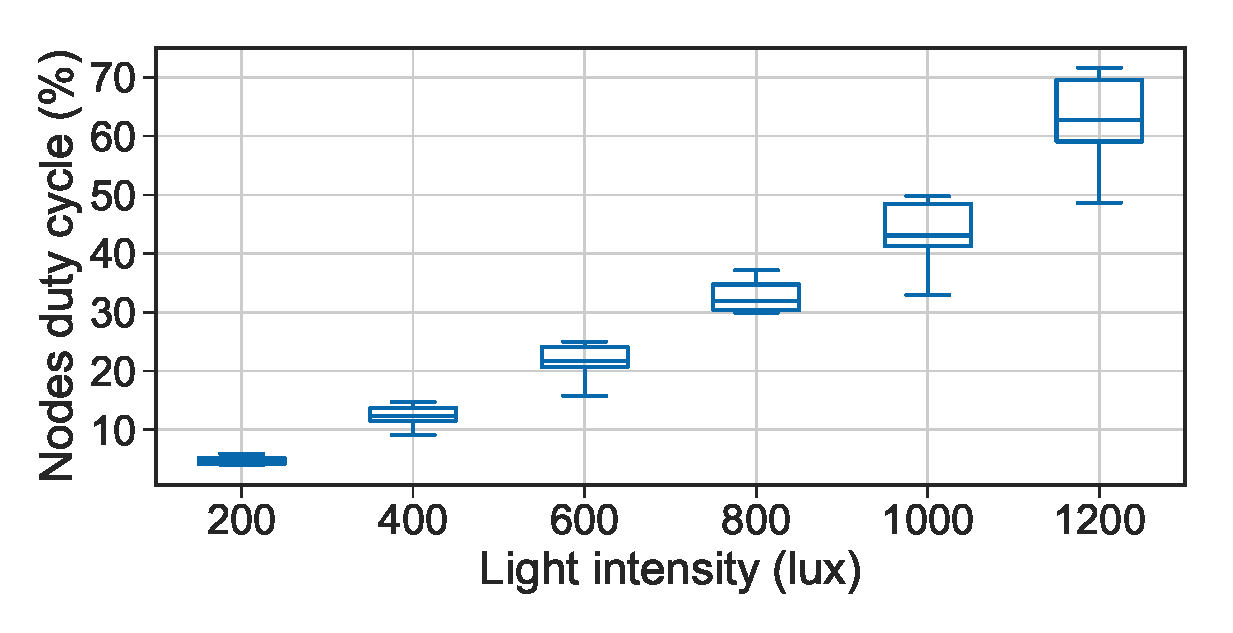
\includegraphics[width=\textwidth]{figures/cis_dutyCycle}
			\caption{Light}
		\end{subfigure}\hfill
		\begin{subfigure}{.49\columnwidth}
			\centering
			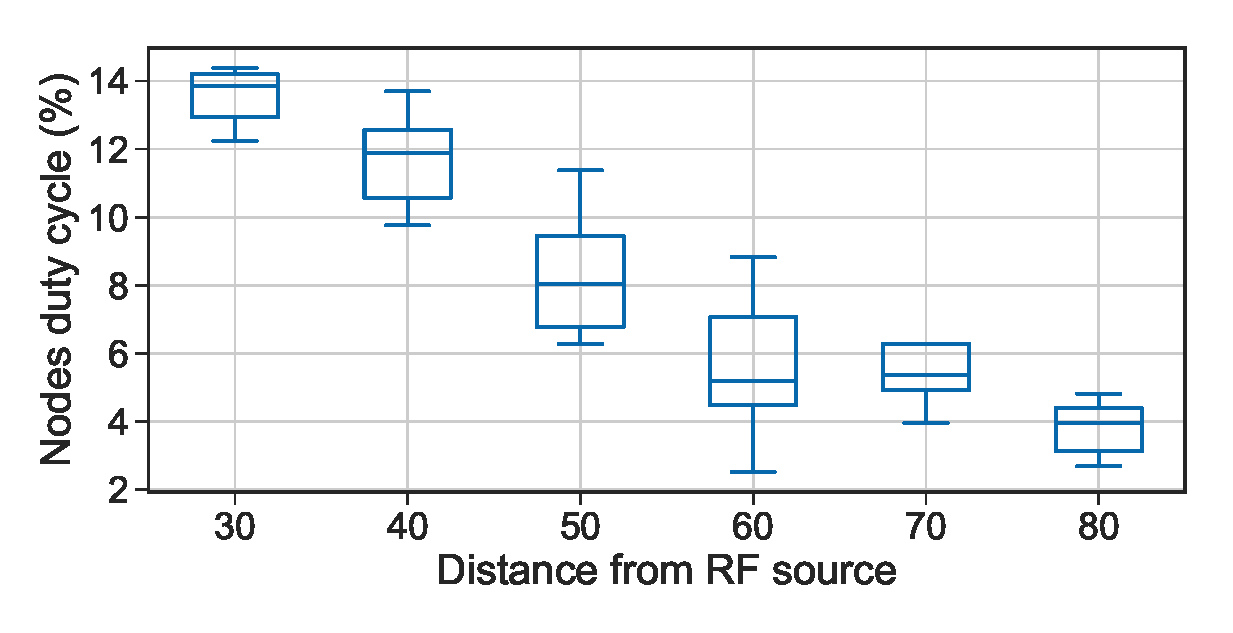
\includegraphics[width=\textwidth]{figures/rf_cis_dutyCycle}
			\caption{RF}
		\end{subfigure}\hfill
		\caption{The average duty cycles of 8 solar-powered and 6 RF-powered intermittent nodes for different ambient energy sources and energy intensities. In general, the average duty cycle of a node is a good indicator of the average duty cycle of the other \cis nodes.}
		\label{fig:cis_nodes_dutyCycle}
\end{figure} 

% In order for a node to estimate the number of active nodes at a given moment, first, it has to know the total number of nodes ($N$) in its \cis, which we assume to be known to the nodes before deployment. Second, this analysis is built on the observation that a node's on-time is a good indicator about the on-times of other nodes in the \cis, see Figure~\ref{fig:cis_nodes_dutyCycle}. A node can measure its on-time $t_\text{on}$ and off-time $t_\text{off}$ using  Algorithm~\ref{algo:offTime} (or an external dedicated timer~\cite{hester2017timely}). 

To estimate the number of active nodes, a \cis node needs to determine the following information:
\begin{enumerate*}[label=(\roman*)]
 \item the total number of nodes in its \cis, which is a typically constant value that can be loaded to the device memory; 
  \item the on-times distribution, which is uniform in our case; and
 \item its own average $\overline{t_\text{on}}$ and $\overline{t_\text{off}}$. 
\end{enumerate*}

Since, we assume that a \cis nodes have the same energy buffers and are in the vicinity of each other (thus, they are exposed to the same energy conditions) then their duty cycles should approach the same value. 
Figure~\ref{fig:cis_nodes_dutyCycle} shows the average duty cycles of the nodes of a solar- and RF-powered \cis{}s. In general, we can conclude that a node's average duty cycle is a good estimator of other \cis nodes' duty cycles.
% We can conclude from these measurements that a node power cycle approximates other \cis nodes power cycles.
% This observation can be generalized by considering that the nodes of a \cis are assumed to have the same energy buffer size and they are in a close proximate, and therefore, they are expose to roughly the same energy conditions 
% (this should not be confused with argument about the emerging uniform distribution of nodes' on-times as this distribution appears due to \emph{small} differences between the power cycles).  
Now, a node can estimate the maximum time span, $t_\text{max}$, of its \cis, which is the total duration of the nodes' on-times when they are aligned next to each other, as follows
\begin{equation}
t_\text{max} = N\times \overline{t_\text{on}}.
		\label{eq:max_time}
\end{equation}
Then, from equation~\ref{eq:cisModel}, the node calculates the \cis availability, $A_\text{v}(N)$. As we argued in Section~\ref{subSec:availability}, nodes on-times are uniformly distributed; therefore, the overlapping on-time is also uniformly distributed. As such, a node can calculate the average number of active intermittent nodes, $N_\text{active}$, using the following formula,
\begin{equation}
	N_\text{active} = \frac{t_\text{max}}{\overline{t_\text{p}}\times A_\text{v}(N)}.
	\label{eq:active}
\end{equation}

\subsubsection{Response randomization factor}

Once a node has estimated the number of active neighbors, $N_\text{active}$, it can use the following formula to determine the response probability,  

\begin{equation}
	P_\text{resp} = 
	\begin{cases}
		\frac{N_\text{resp}}{N_\text{active}} & \ \  \text{if} \frac{N_\text{resp}}{N_\text{active}} < 1\\
		1 									  & \ \ \text{otherwise},
	\end{cases}
	\label{eq:randFactor}
\end{equation}

where $N_\text{resp}$ is a system parameter that reflects the desired redundancy factor required by an application. 

% and choose the proper randomization factor. If a second event, however, happens shortly after the first one, a node needs to update $N$ as follows, 
% $$
% N = N - (N_\text{active}-1)
% $$
% the $-1$ is because the node itself decided not to react on the first event. 

Table~\ref{tab:clusters} shows the average number of active nodes of an 8-nodes \cis for different light intensities. These measurements provide a sanity check on equation~\ref{eq:active}. For example, at $\SI{1200}{lux}$ an individual node of our \cis has a duty cycle of $\approx$\,62\%, i.e., it is on average 0.62\,$t_\text{p}$ operating. If we multiply that by the number of nodes (equation~\ref{eq:max_time}) we get about 5\,$t_\text{p}$. Figure~\ref{fig:cisModel} indicates that a \cis with eight nodes of duty cycles above 50\% has near 100\% availability. From equation~\ref{eq:active}, we find that the expected number of clustered nodes is 5 confirmed by the measurements presented in Table~\ref{tab:clusters}. 


\begin{table}
		\centering
		\caption{Measuring intermittent nodes overlapping of a \cis of 8 intermittent nodes for different light intensities.}
		\begin{tabular}{llll}
				\hline
				\textbf{light (lux)} &\textbf{on/off cycle (\%)}  & \textbf{$N_\text{active}$} & \textbf{std}   \\
				\hline
				\ \ 300	                 & \ \ 8  & 1.01 & 0.85   \\
				\ \ 500                  & 17 & 1.63 & 0.98   \\
				\ \ 800                  & 31 & 2.88 & 1.50   \\
				1200                 & 62 & 5.05 & 1.08   \\
				\hline
		\end{tabular}
		\label{tab:clusters}
\end{table}








































%\section{Distributed Intermittent System} 
\section{Prototype: Coalesced Intermittent Command Recognizer}
\label{sec:disMic}
\begin{figure}
	\centering
	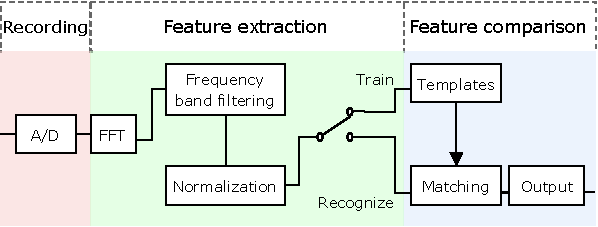
\includegraphics[width=\columnwidth]{figures/cis}
	\caption{\fullCIM: an instant of a \fullsys. \cim features a power failure immune word recognizer. Once a word is recorded, the word's spectral features extraction begins. The resulting features vector is compared against previously-stored words' templates for recognition. The comparison using a liner distance matching algorithm}
	\label{fig:cis}
\end{figure}

We have developed a prototype of a \fullcim (\cim): an instant of a \fullsys. The \cim consists of eight batteryless intermittent nodes. Each node is capable of performing isolated words recognition. 

The reason behind developing a \cim is threefold: (i) voice is a natural and convenient way for human to interact with miniaturized devices; (ii) demonstrating \textit{the world's first} batteryless intermittently-powered command recognizer, which shades light on the potential of batteryless intermittent systems; and (iii) facilitating testing with different sensing strategies and different type of external events arrival (i.e. regular  or burst). 

Moreover, we believe that a \cim can facilitate direct human-to-human or human-to-objects communication. Imagine that a \cim based system is deployed in a play ground, embedded in ground and other objects. You want to call your child, and a \cim based system is embedded in your shirt and his shirt. You say his name and the \cim picks up the word and scatter it over light---\cite{marco} demonstrates the feasibility of scattering sunlight to communicate between two nodes that are up to 60\,m apart. The scattered signal will be relied on other \cim nodes until the receiving node on his shirt receives the message and notify him, daddy is calling. 

\subsection{Hardware}
A \cim node consists of thee main parts: a microphone, a microcontroller, and a harvester. MSP430RF5994~\cite{ti_msp430_website} an ultra-low-power microcontroller is used for data acquisition and processing. This microcontroller has a 16-bit RISC processor running on 1 MHz, 8KB of SRAM (volatile), 256KB of FRAM (non-volatile), and a 12-bit analog to digital converter (ADC). It also features a Low Energy Accelerator (LEA), which offloads the main CPU for specific operations, such as FFT. For recording we use the PMM-3738-VM1010-R piezoelectric MEMS microphone, which features Wake on Sound and ZeroPower listening technologies \cite{microphone}, allowing both the microcontroller and the microphone to sleep in a low-power mode until a sound wave is detected.
The microcontroller and microphone are powered by a BQ25570 solar power harvester~\cite{BQ25570EVM-206_website} connected to an IXYS SLMD121H04L solar cell~\cite{SLMD121H04L_website} and a super-capacitor of 470 \si{\micro F}. For debugging we used the Saleae logic analyzer~\cite{saleae}.

\subsection{System Description}
The \cim has a power interrupts immune command recognizer. The recognizer is capable of recognizing isolated-word type of speech. 
The main parts of the recognizer are illustrated in Figure~\ref{fig:cis} and explained below:

\subsubsection{Data acquisition}
The \textit{Wake-on-Sound} feature of the microphone triggers the data acquisition process once the energy level in the sound signal crosses a certain level. The ADC, then, samples the output of the microphone at 7,812\,Hz. This sampling rate is sufficient to cover most of the frequency range of the human voice. To determine the end of the recording we relied on the characteristics of the targeted vocabulary. In particular, we identified, experimentally, the minimum effective recording length, which is happened be 259\,ms for the chosen set of words. By exploiting the Wake-on-Sound feature and the minimum effective recording length we eliminate the need for an endpoint detection algorithm~\cite{}, greatly improving the processing time and system efficiency from the energy perspective.


\subsubsection{Feature Extraction}
Once a recording has finished, framing and data processing begin. \cim divides the digitized signal into non-overlapping frames of 256 samples ($\approx$ 33 milliseconds). This size is beneficial for doing a Fast Fourier Transform and short enough for the voice-features to be considered constant inside a frame.

To extract the spectral features of a frame, \cim divides the frequency of interest into 12 bands (as in~\cite{hopper1992}). The first five bands has a bandwidth of 200\,Hz. The next three has a bandwidth of 300\,Hz which is followed by two bands of 500\,Hzs. Finally, the last two bands has a 600\,Hz bandwidth. This division is motivated by how the energy is concentrated in human speech~\cite{hopper1992}. Then, \cim computes the 256-point Fast Fourier Transform for each frame. The resulting feature vector contains the amount of energy concentrated in each frequency band defined earlier. This feature vector forms the basis for the words identifying process once it is normalized.

Normalization minimizing detection errors that result from differences in the amplitude of the speech input of a word. To normalize a feature vector, \cim computes the binary algorithm of each entry of that vector. 
Then it computes the mean of the resulting vector. Finally, it subtracts each entry of the resulting vector from the computed mean. This is summarized in the following equation: 
\begin{equation}
    f_i = \log(\hat{f}_i) - \frac{\sum\limits^S_{i=1}\log(\hat{f}_i)}{S},
\end{equation}
where $f_i$ is the normalized output for the $i^{\text{\tiny th}}$ spectral band of a feature vector, $\hat{f}_i$ is the energy in the $i^{\text{\tiny th}}$ spectral band of the frame, and $S$ is the number of spectral bands (12 in our case). 

\subsubsection{Feature Matching}
Feature matching is done by computing the distances between the normalized feature vectors of the recorded word and the vectors of the words stored during the training phase. 
\cim computes the squared Euclidean distance between vectors as follows,
\begin{equation}
	 	d_j = \sum\limits^S_{i=1} (f_{s,i} - f_{r,i})^2,
    \label{eq:frame_dist}
\end{equation}
where $d_j$ is the distance between the $j^{\text{\tiny th}}$ stored and recorded vectors. $f_{s,i}$ is the normalized output of the $i^{\text{\tiny th}}$ spectral band of a stored vector, $f_{r,i}$ is the normalized output of the $i^{\text{\tiny th}}$ spectral band of a recorded vector. 
The total distance between two words is calculated as follows:
\begin{equation}
		D_k = \sum\limits^{l}_{j=1} d(j)
\end{equation}
where $D_k$ is the distance between the $k^{\text{\tiny th}}$ stored word and the recorded word, and $l$ is the recording length measured in frames.

Once the recorded word has been compared to all \cim dictionary words, the word with the smallest distance to the recorded word is considered the correct word. However, if the smallest distance is bigger the garbage threshold \todo{Partick uses confusion matrix for setting this threshold. Maybe I need to consider adding it} which we experimentally set, then the \cim will return "undefined word". 

It should be emphasized that in Linear distance matching (LDM) the feature vectors of two words are compared successively, not accounting for differences in pronunciation speed. This is sufficient for our case as we are targeting isolated words and speaker dependent speech recognition type\footnote{We have also implemented Dynamic Time Warping algorithm which better handles the difference in the speed of speech. However, it is slower than the linear matching algorithm and the detection accuracy were comparable in our case}. 

\subsubsection{Power Failure Protection}
In order to preserve the progress state and to protect \cim data against randomly timed power failures, we manually splitted \cim program into 19 atomic regions. We ensured the each of these regions requires less energy the what the energy buffer can provide with a single charge. The program progress state is saved in the non-volatile memory (FRAM) on the transition between these regions. This prevents the program from falling back to its starting point (\texttt{mian()}) after each power failure. Data in the non-volatile memory with Write-After-Read dependency are double buffered to ensure the data integrity when the power supply is interrupted. 

\subsection{Code profiling}
The entire command recognition software was written in the {\tt C} programming language. The total program consists of 973 lines of code, excluding the Texas Instrument DSP library, from which the FFT function was used. See \ref{tab:code_stats} for more information.

The memory footprint on the microcontroller was 20,064 bytes of FRAM and 1,134 bytes of SRAM. Execution times are shown in \ref{tab:profiling}.

The power usage of a node differs according to it's activity. When a node is waiting for a voice event, it is in low-power mode. When data needs to be processed or recorded it is in active mode. When recording, the microphone and ADC consume additional power. The power consumption rates are measured with a Monsoon power monitor~\cite{monsoon} and shown in \ref{tab:power_usage}.


\begin{table}
	\centering
	\caption{Code statistics: lines of code}
	\label{tab:code_stats}
	%Compiled without optimization flags:
	\begin{tabular}{lrrrr} \hline
		Language & Files & Blank & Comment & Code \\\hline
		C & 7 & 264 & 173 & 736 \\
		C/C++ Header & 8 & 62 & 40 & 237 \\\hline
		Total &  15 & 326 & 213 & 973 \\\hline
	\end{tabular}
\end{table}

\begin{table}
	\centering
	\caption{Power usage.}
	\label{tab:power_usage}
	%Compiled without optimization flags:
	\begin{tabular}{lrrr}\hline
	Section & Current (\si{\micro A}) & Voltage (V) &  Power (\si{\micro W}) \\\hline
	Sleeping & 64 $\pm$20 & 2.008 $\pm$? & 128 $\pm$40 \\
	Recording & 423 $\pm$20  & 2.008 $\pm$? &  849 $\pm$40\\
	Processing &  282 $\pm$20 & 2.008 $\pm$?& 566 $\pm$40 \\\hline
	\end{tabular}
\end{table}

\clearpage


\section{Evaluation}
\label{sec:evaluation}
\begin{figure*}[h]
        \begin{subfigure}{.66\columnwidth}
            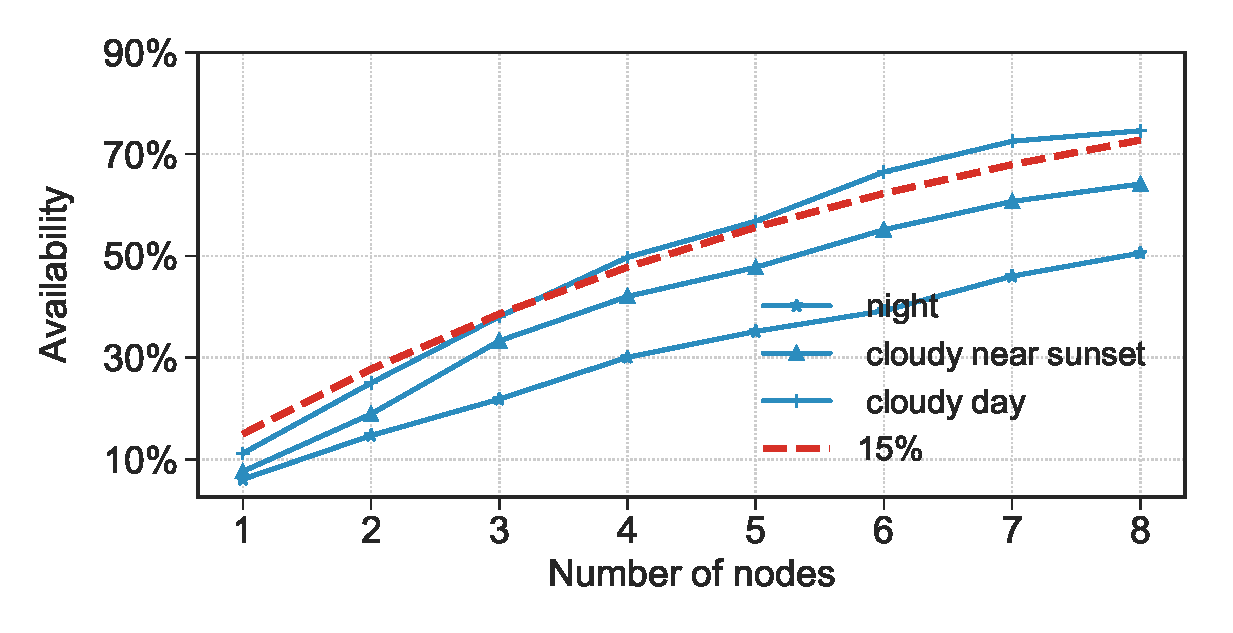
\includegraphics[width=\textwidth]{figures/sysAvailability}
                \caption{The \cis is powered by uncontrollable light sources---artificial light (night) and sunlight (day).}
            \label{fig:solarPwrCIS}
        \end{subfigure}\hfill
        \begin{subfigure}{.66\columnwidth}
            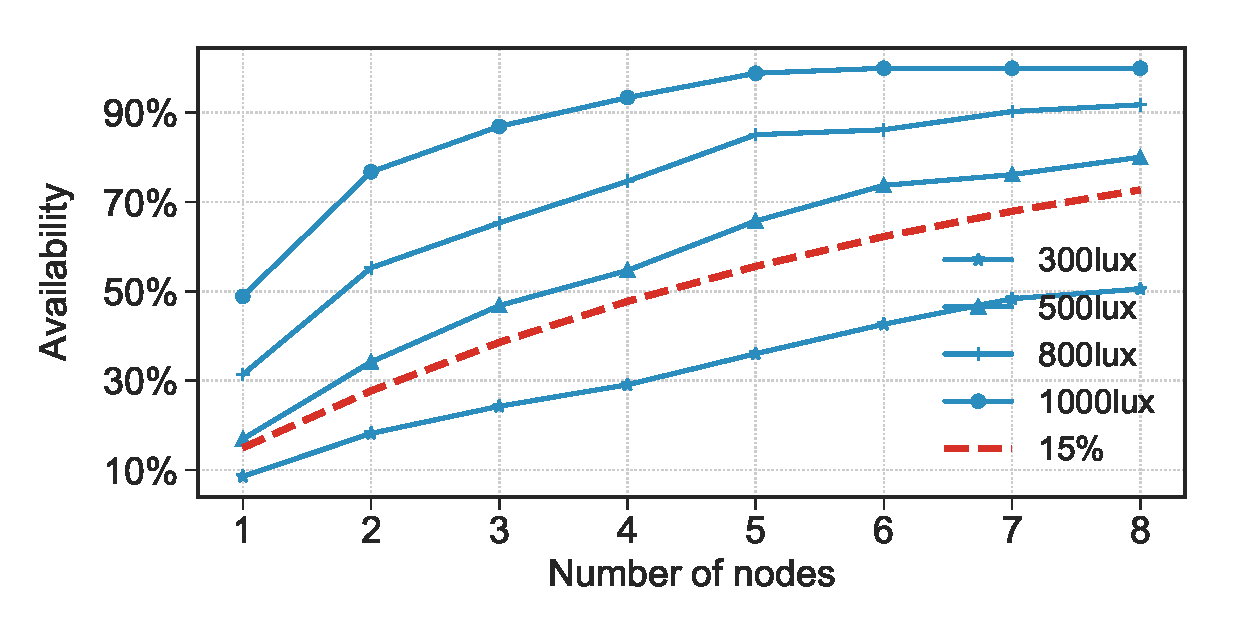
\includegraphics[width=\textwidth]{figures/sysAvailability_artificial-light}
                \caption{The \cis is powered by a controllable array of LEDs. \vspace{1em}}
            \label{fig:artPwrCIS}
        \end{subfigure}\hfill
        \begin{subfigure}{.66\columnwidth}
            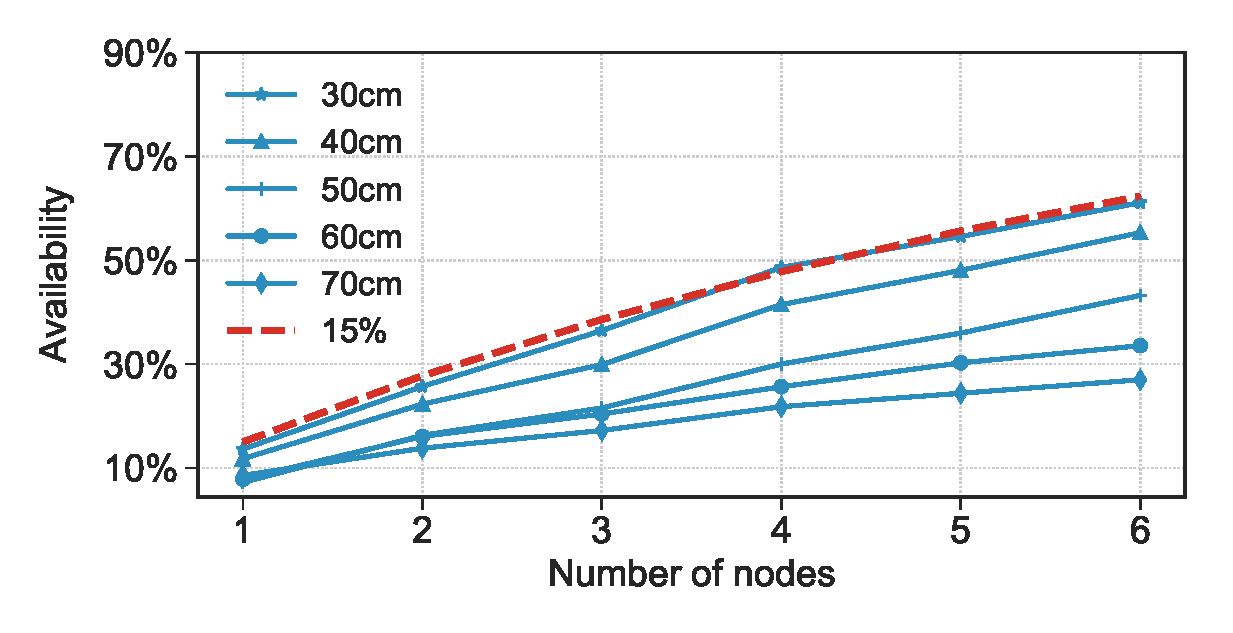
\includegraphics[width=\textwidth]{figures/rf_sysAvailability}
                \caption{The \cis is powered by an RF reader~\cite{r420_website} located 30-70\,cm away from the RF tags (WISPs~\cite{smith2006wirelessly}).}
            \label{fig:rfPwrCIS}
        \end{subfigure}
        \caption{The \fullcis's availability for differed energy sources and number of nodes. 
        The modeled availability (represented by dashed lines with nodes' duty cycles of 15\%) approximates the measured availability with high accuracy.}
        \label{fig:pwrCIS}
\end{figure*} 
To evaluate the performance (availability) of the \fullcis, we conducted several experiments in different energy conditions and with different event arrivals patterns. 
%
\subsection{Availability}
%%%%%%%%%% ToDo %%%%%%%%%%
% Experiment setup
Irrespective of the energy source (RF or light) we showed in Figure~\ref{fig:power_cycles} that the power cycles of a \cis's nodes are different, which leads to a uniform distribution of their on-times, as we argued in Section~\ref{subSec:availability}. We captured the expected joined availability of these nodes in Model~\ref{eq:cisModel}.  Here, we validate model by comparing the modeled availability of a \cis against data captured with different hardware (solar- and RF-powered nodes) in different scenarios.
% the measured ones under different powering conditions and with different hardware. 
 
Figure~\ref{fig:pwrCIS} shows the availability of three \cis{}s when they are powered by sunlight, artificial light, and RF and for a different number of intermittent nodes.
%%%%%%%%%% ToDo %%%%%%%%%%
% clarify that the RF and solar power nodes use different hardware.
The results clearly confirm our expectation: when the power cycles are slightly different, the on-times are uniformly distributed. The results also validate our model; the dashed lines represent the modeled availability when the nodes duty cycle is 15\%.

\subsubsection{Availability on a Fine Scale}
%
\begin{figure}[t]
    \centering
     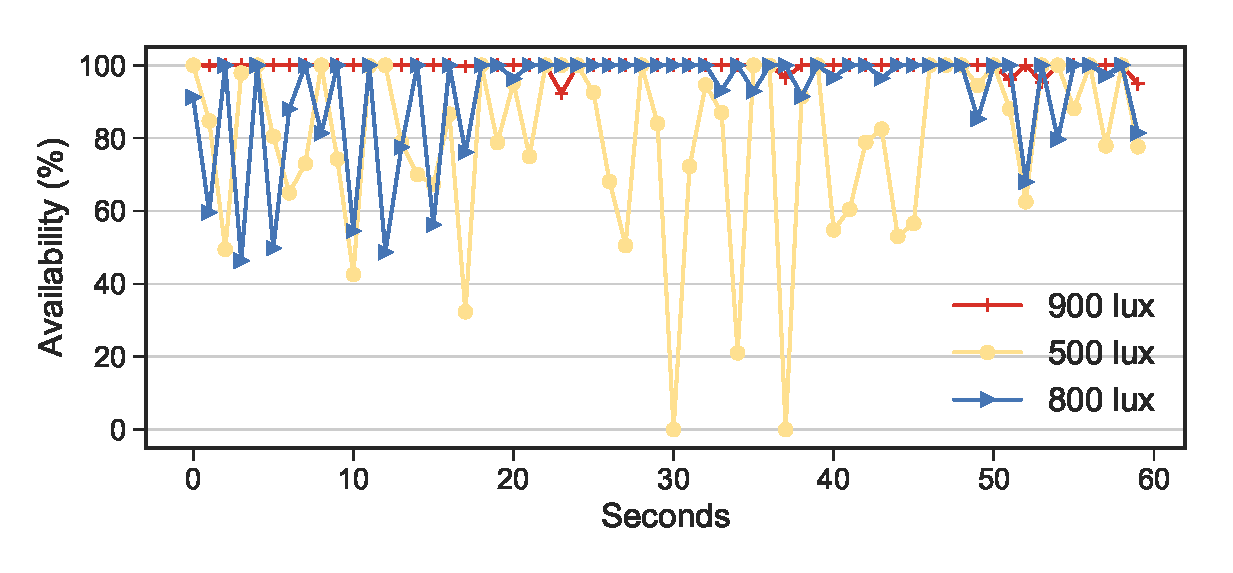
\includegraphics[width=\columnwidth]{figures/sysAvailabilityTimeline_470_sleep_5seconds_2}
    \caption{\cis availability observed with a 5 seconds time window.}
    \label{fig:fineScaleAvailability}
\end{figure}
% In Section~\ref{subSec:availability}, we discussed that the \cis availability is not a constant value. 
Since the nodes' on-times are in a constant shift relative to each other (Section~\ref{subSec:availability}), the collective availability of the \cis fluctuates when it is observed in a short time window. 
Figure~\ref{fig:fineScaleAvailability} captures \cis availability on a time window of 5 seconds for thee different ambient energy conditions. In these experiments, the average power cycles of the \cis's nodes are (3,18), (3.9,12.3), and (4.3,11.5) seconds when ambient light intensity are 500, 800, and 900\,$\si{lux}$, respectively. 
If we focus on the line graphs associated with 500 and 800\,$\si{lux}$ and compare the system availability within the interval $[20,50]$ seconds and the rest, we can observe that the \cis gradually alternates between low and high collective availability; nodes' on-times gradually transition from maximum to minimum separation and vice versa (Section~\ref{subSec:availability}). Notice that, when ambient light intensity was 800\,$\si{lux}$ the \cis collective availability transited from low to high to low, while this pattern happened to be reversed when light intensity was  500\,$\si{lux}$. For the 900\,$\si{lux}$ the 8-node \cis achieved near-continuous $100\%$ availability. 
%
% \begin{table}
%     \centering
%     \caption{The \cis availability on fine scale: the effect of the energy buffer size and the time interval within a \cis is observed on the system availability}
%     \label{tab:availFineScale}
%     \begin{tabular}{r|l|l|l|r}
%     \hline
%     Intervals (sec) & -    & RF ($47\si{\mu F}$)      & -    & light ($470\si{\mu F}$)  \\ 
%     \hline
%     -             & mean  & std     & mean     & std   \\ \hline
%     0.5             & 61    & 8.8     & 27.3     & 42.9   \\
%     1               & 61    & 5.9     & 27.3     & 41.5   \\
%     2               & 61    & 4.4     & 27.3     & 37.5   \\
%     \hline
%     \end{tabular}
% \end{table}

% Table~\ref{tab:availFineScale} captures the \cis availability on fine scale. An obvious but important observation is that the \cis availability flactuates, see the std columns.    for two different energy buffer sizes. 


% \begin{table}
%     \centering
%     \caption{The \cis availability on fine scale: the effect of the energy buffer size and the time interval within a \cis is observed on the system availability}
%     \label{tab:availFineScale}
%     \begin{tabular}{r|l|l|l|r}
%     \hline
%     Energy Intensity & -    & RF ($47\si{\mu F}$)      & -    & light ($470\si{\mu F}$)  \\ 
%     \hline
%     -             & mean  & std     & mean     & std   \\ \hline
%     high          & 61    & 8.8     & 91.3     & 24.9   \\
%     medium        & 43    & 7.4     & 67.6     & 44.3   \\
%     how           & 21    & 3.4     & 27.3     & 37.5   \\
%     \hline
%     \end{tabular}
% \end{table}




\subsection{Sensing}
\subsubsection{Experiment setup}
\label{sec:experiment_setup}
% \paragraph{availability on a fine scale}
 % \todo{Because of the differences in intermittent nodes power cycles, their duty cycles are constantly shifting relative to each other ( Figure~\ref{fig:cisOntime}).  However, this study does zoom in on the \cis availability on short time scale and the effect of length of the differences between the nodes power cycles on the system short term availability. } 
%
After validating our observation on different energy sources, we designed a testbed with controllable light intensity for clarity and reproducibility. To this end, we blocked uncontrollable light sources with a box of $60 \times 40 \times 40$\,cm. On the box ceiling, we attached a light strip of 2.5\,m with 150 LEDs that can produce 15 different light intensities. On the bottom a \fullCIM of 8 intermittent nodes is placed (see Section~\ref{sec:hardware} for hardware description).

The events in our experiments are spoken words (Table~\ref{tab:words}). 
Short events (see events classification in Section~\ref{sec:event_classification}) are represented with individual words, while burst events are represented with phrases of a few words.
We recorded different patterns of inter-event and inter-bust arriving time. We used a Bluetooth speaker~\cite{jbl} to replay a certain recording. 
% The data were collected using a logic analyzer~\cite{saleae} and processed on a laptop running Ubuntu 16.04 LTS. 
%
\subsubsection{Events detection rate}
%
\begin{figure}[t!]
		\centering
	    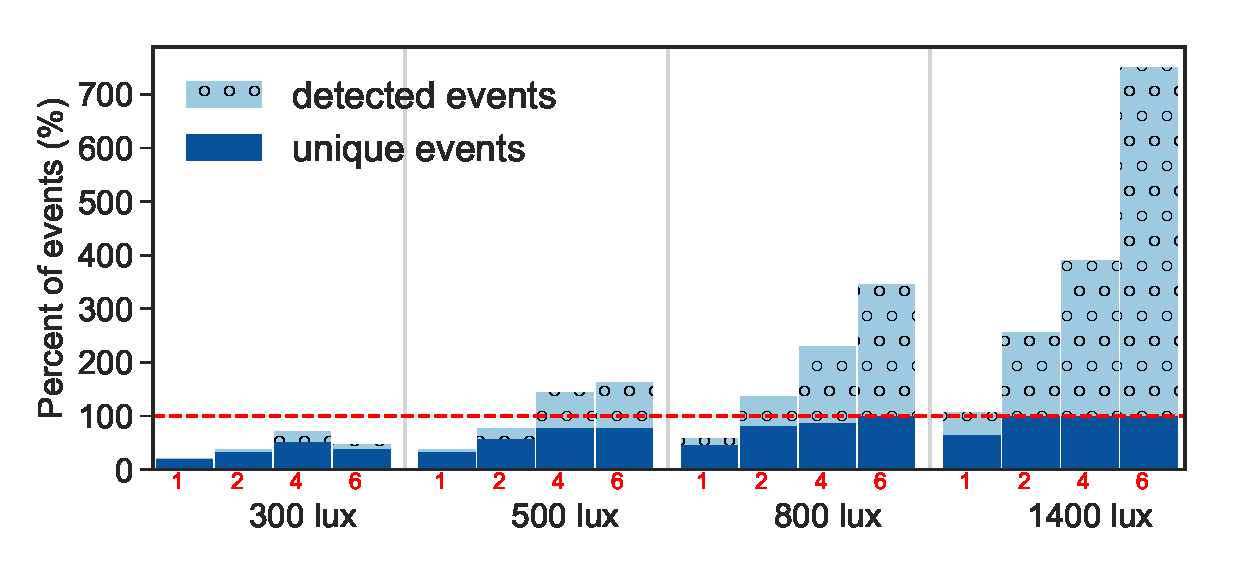
\includegraphics[width=\columnwidth]{figures/regular_events_capture_rate_2.eps}
		\caption{Duplicate and unique events captured by a \fullcim of eight solar-powered nodes. In general, the number of captured events increases in two case: when light intensity rises and when inter-event arrival time increases. 
         % In general, we see that when the light intensity increases, the number of detected and captured events rise too. Moreover, there is a positive correlation between the length of the inter-event arrival time and the detection and capture rates. 
         Red numbers indicate events arrival interval in seconds.
         }
    	\label{fig:events_detection_rate}
\end{figure} 
Here we experiment with the behavior of a \cis when events arrive individually or in bursts \emph{without} enabling  randomized response in favorable energy conditions. 
%
\begin{figure}[t]
    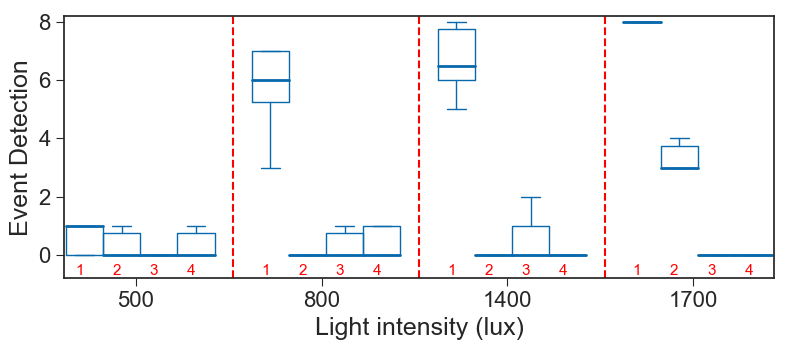
\includegraphics[width=\columnwidth]{figures/events_burst_problem_2}
	\caption{When capturing a burst of 4 events without randomizing the response, the majority of the nodes react to the first event in the burst and power down shortly after, missing the rest of the burst.}
    \label{fig:events_burst_problem}
\end{figure}
%
\paragraph{Individual events.}
\begin{figure}[t]
	\centering
     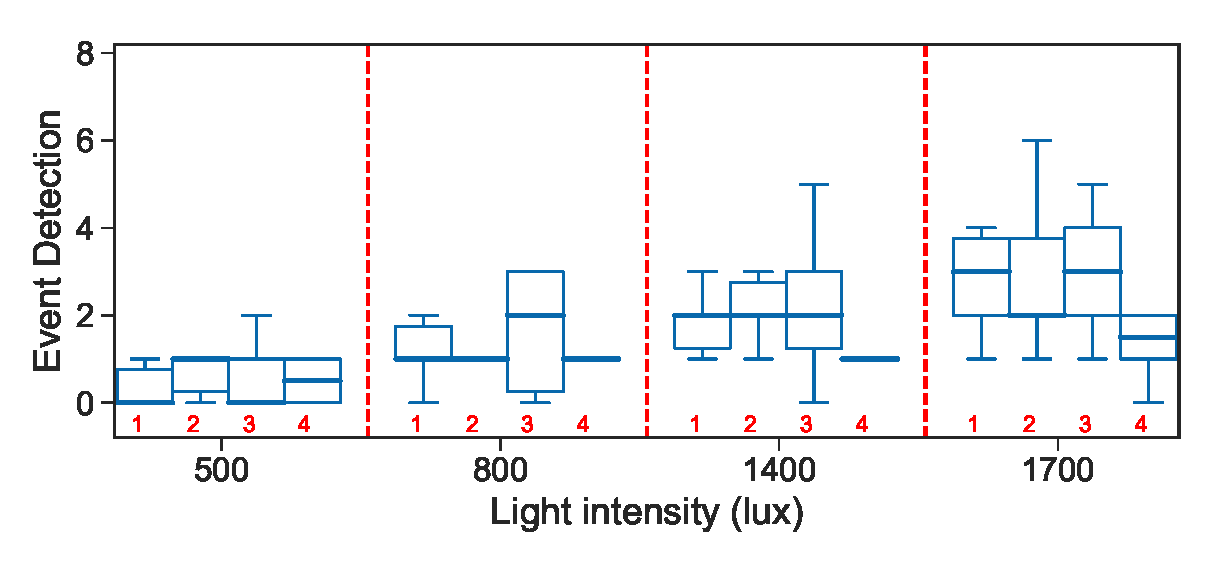
\includegraphics[width=\columnwidth]{figures/events_burst_rand_2}
    \caption{Response randomization enables a \cis to capture the entire burst of events with high capturing rates. It also reduces the number of duplicated events. Red numbers indicate events index in a burst.}
    \label{fig:events_burst_rand}
\end{figure}

Figure~\ref{fig:events_detection_rate} shows the percentages of capturing duplicate and unique events when light intensity varies from $\SI{300}{lux}$ to $\SI{1400}{lux}$ and the inter-event arrival time ranges from $\SI{1}{second}$ to $\SI{6}{seconds}$. For each experimental trial 20 words were played, resulting in a total of 240 playbacks. 

Figure~\ref{fig:events_detection_rate} shows a positive correlation between light intensity and the number of detected events. In particular, the number of duplicate detections rises dramatically when light intensity increases, \emph{demonstrating the overpowering problem} (Section~\ref{sec:power_state}). Moreover, increasing the inter-event arrival time also surges the number of duplicated events. The reason for this is that when the time between events increases, the intermittent nodes get the chance to sleep longer in low-power mode, consuming less energy. Thus, nodes' on-times expand, reducing their inherent randomization, which leads them to be in \textit{hibernating power state} (Section~\ref{it:hibernating}).  

% Indirectly, these results show how a \cis can achieve a much higher duty cycle than its individual intermittent nodes: Figure~\ref{fig:cis_nodes_dutyCycle} shows that with a light intensity of $\SI{800}{lux}$ an intermittent node is active with a duty cycle of 30\% while Figure~\ref{fig:events_detection_rate} shows that a \cis of 8 nodes captures 100\% of the unique events when the time between them is \SI{6}{s}. 

\textit{Bursty events.}
Figure~\ref{fig:events_burst_problem} shows the capturing behavior of a \cis when the events arrive in bursts. A burst of four events with one second between the individual events was fired every 20 seconds. Each burst was repeated 10 times and under four different light intensities. The nodes sleep in a low-power mode when they finish processing an event, waiting for the next one. 

In general, we observe that in favorable energy conditions (above $\SI{500}{lux}$) intermittent nodes react to the first event of a burst and power down shortly after, missing the rest of the burst. These results confirm our argument about the side effect of the \textit{hibernating power state} of a \cis (Section~\ref{sec:power_state}). These results also demonstrate that the hibernating power problem happens on a wide range of power intensities, showing its significance. Next, we will show how randomizing the response can mitigate the problems generated when ambient energy exceeds the design point. 

\subsubsection{Events detection rate with randomization}
\begin{table}
	\centering
    $
    \begin{array}{llll}\hline
     \textbf{(lux,second)} & \textbf{(800,6)} & \textbf{(1400,4)} & \textbf{(1400,6)}\\\hline
    \textit{randomization}    & 205/432 &  236/675 & 223/493 \\
    \textit{no randomization} & 240/831 &  240/938 & 240/1802 \\\hline
    \end{array}
    $
    \caption{These results are presented as \textit{unique/total} detected events. A node response probability is 65\% in the first two scenarios,\textbf{(800,6)} and \textbf{(1400,4)}, and 30\% in the last one.   
    Randomizing the response reduces the number of duplicated events by 50\% while losing only 7\% of the unique events.}
    \label{tab:regular_rand}
\end{table}
% 
Here, we examine the effect of enabling artificial randomization on the \cis's response. 

\paragraph{Individual events.} 
Table~\ref{tab:regular_rand} compares the number of detected events when the \cim's response is randomized and not randomized.
When randomization is enabled, nodes respond to events with a probability of 65\% for the scenario of $\left(\SI{800}{lux}, \SI{6}{seconds}\right)$ and $\left(\SI{1400}{lux}, \SI{4}{seconds}\right)$, and for the highest energy level and the longest inter-event arrival time the responding probability was set to 30\%.

Table~\ref{tab:regular_rand} shows that randomizing the response reduces duplicated events by an average of $\approx$50\%, while only marginally lowers the number of the uniquely detected events (7\% on average). 


\paragraph{Bursty events.}
To enable a \cis to capture events arrive in bursts, the response probability for each events in a burst should be different. The \cis should respond with a minimum probability to the first event in a burst and gradually increase the response probability for the subsequent events in the burst (we assume that between the bursts the \cis resumes to its expected collective availability). This gradual increment to the responding probability is motivated by the observation that when a node captures an event it becomes unavailable for the subsequent ones in the burst.
In this experiment, the nodes reacted with a probability of 40\%, 50\%, 70\% and, 100\% on the first, second, third and fourth event, respectively. Since the event distribution is known these probabilities were fixed during the development stage.

Figure~\ref{fig:events_burst_rand} shows how randomizing the \cis response spreads the nodes' awake times--as compared to Figure~\ref{fig:events_burst_problem}--and enables the \cis to capture the entire burst with a high probability, i.e., above 85\%. 
% Additionally, we also observe a positive impact of randomizing the response when the system is under-powered ($\SI{500}{lux}$).

%40 50 70 100


% \subsection{Coalesced intermittent command recognizer word detection accuracy}
% For evaluating the \fullcim accuracy, we used the word set in Table~\ref{tab:words}.
% Each word was pronounced by a single speaker 20 times and recorded on a PC. One of these recordings was stored as a template on the \cim, while the remaining 19 were played back through a Bluetooth speaker~\cite{microphone} for testing.

% The ratio between detected events and successfully recognized events per node is shown in Figure~\ref{fig:word_freq} and it averages out at  76.7\%. The difference between detection and capture is primarily caused by nodes that have insufficient buffered energy to finish recording.  

% %
% \begin{figure}
% \centering
% 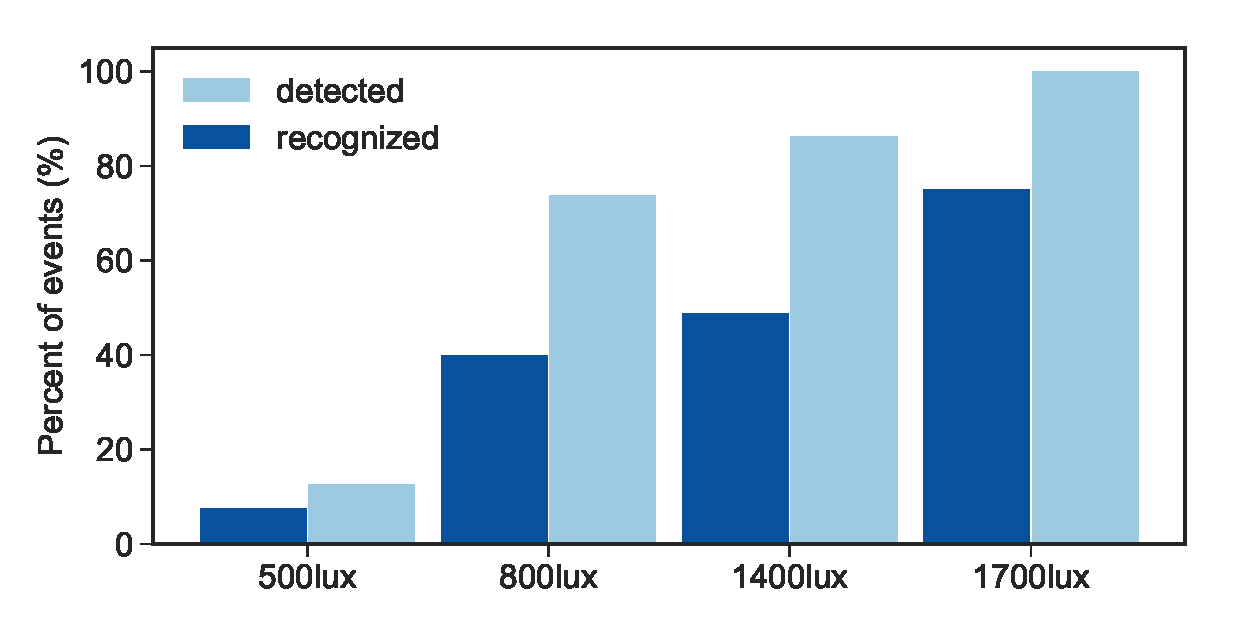
\includegraphics[width=\linewidth]{figures/detection_vs_recognition}
% \caption{
% % The percentage of successfully recognized words as compared to the detected ones.
% The average number of successfully recognized words per node and average number of detected words per node, as percentages of the total number of played words. Words are relatively long events and therefore some of their recordings do not complete due to insufficient harvested energy.}
% \label{fig:word_freq}
% \end{figure}

\begin{figure}
    \begin{subfigure}{0.48\columnwidth}
        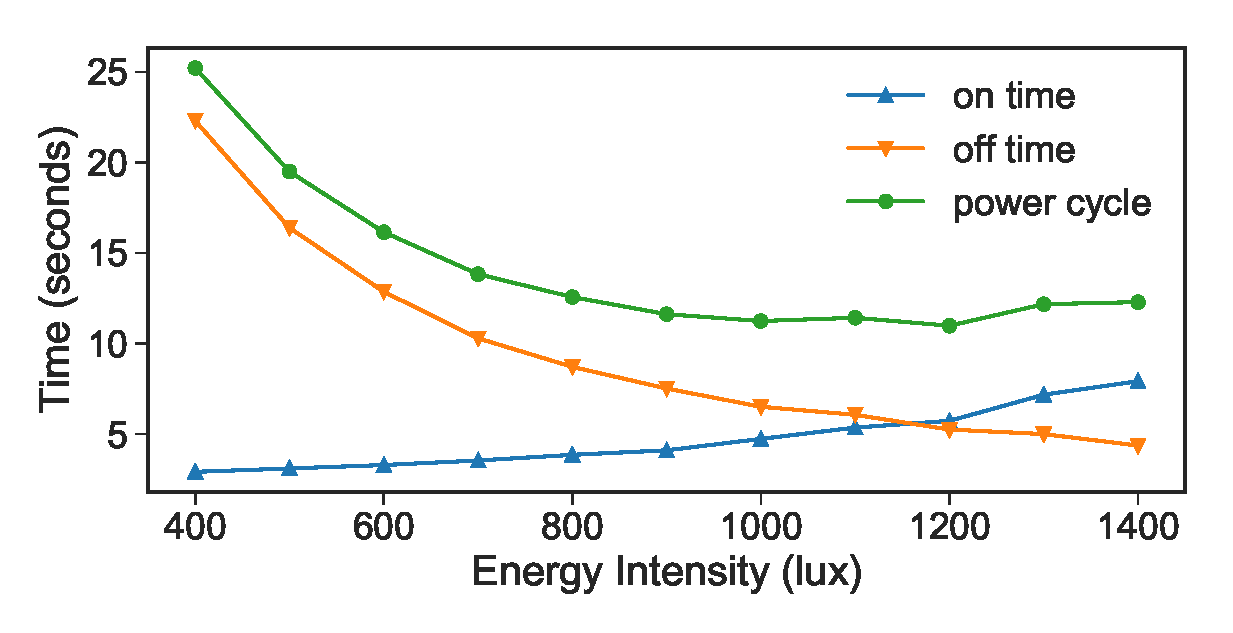
\includegraphics[width=\textwidth]{figures/BatterylessNodesDutyCycles_Sleep_mode}
        \caption{In wake-on-event style of operation, nodes go into low-power mode upon their power-ups. The low power consumption rate at this mode make the on-time of a node an important factor in determining the duty cycle and the power cycle length of the node.}
        \label{fig:differentEnergyIntensity}
    \end{subfigure}\hfill
    %
    \begin{subfigure}{0.48\columnwidth}
        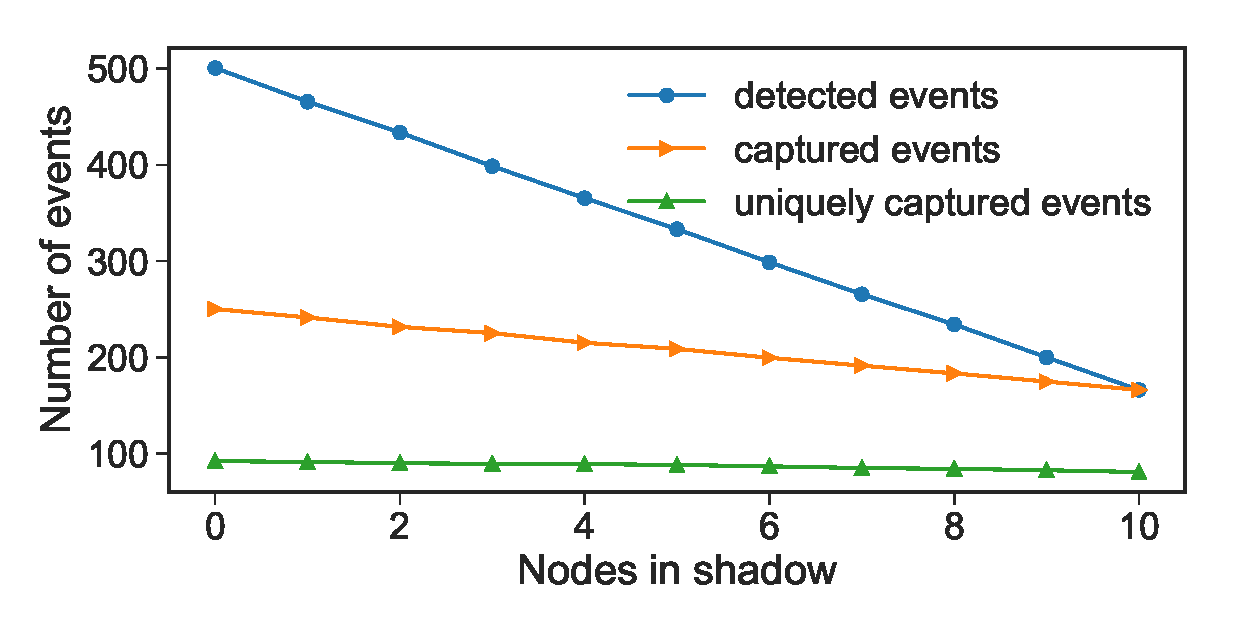
\includegraphics[width=\textwidth]{figures/different_energy_intensity}
        \caption{Simulated results showing how the number of captured events is affected when the shadow is covering a \cis. Detected events are \#times events trigger nodes. Captured events are \#times nodes processed events. We used a redundant factor of 2.5 (see (\ref{eq:randFactor})).}
        \label{fig:sim:differentEnergyIntensity}
    \end{subfigure}
    \vspace{-0.3cm}
    \caption{The effect of non-uniform energy distribution.}
    \label{fig:pwrCycleVSEnergyIntensity}
\end{figure}

\paragraph{Different energy harvesting rates}
It can happen that some of the nodes of a \cis are in the shadow while the rest is under direct sunlight (e.g., when curtains are being opened). 
As a consequence, nodes' power cycles will be significantly different (Figure~\ref{fig:differentEnergyIntensity} shows the on-times, off-times, and power cycles when the ambient energy ranges from 400 to 1400\,lux). Therefore, nodes will not be able to accurately estimate the collective availability of the system. 
%
The inaccurate estimation is most significant when half of the nodes are in shadow. 
However, even during such a worst-case scenario, a \cis availability is not dramatically effected (Figure~\ref{fig:sim:differentEnergyIntensity}). 
This is because half of the nodes will overestimate the availability of the system while the other half will underestimate the \cis's availability.
For example, in these simulation results the node with 50\% duty cycle responded to $\approx$\,50\% of the events while nodes with 16\% duty cycle responded with a probability of 100\%. 
During this simulation, the power cycles, on-time, and off-time of the nodes are 10, 5, and 5 units of time when they are under sunlight and 24, 4, and 20 when they are in shadow. 
The length of the simulated experiment is 1000 units of time and We used a redundant factor of 2.5 (see (\ref{eq:randFactor})).












































% \section{Discussion }
% \label{sec:discussion}
% \begin{figure}
	\begin{subfigure}{0.49\columnwidth}
		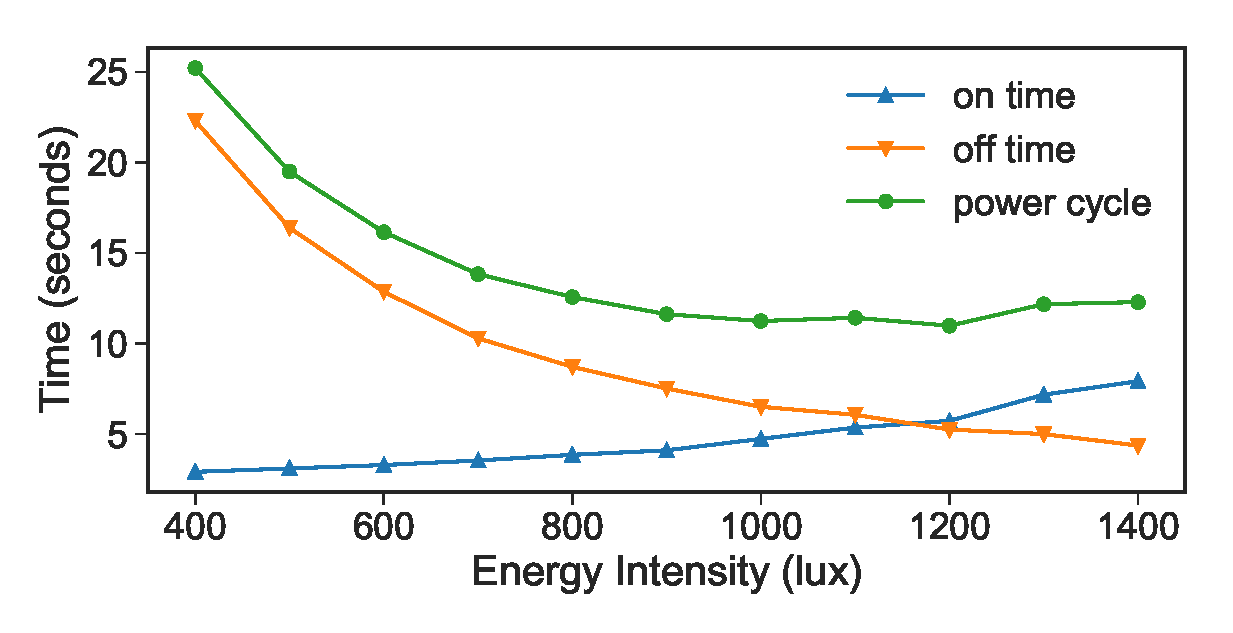
\includegraphics[width=\textwidth]{figures/BatterylessNodesDutyCycles_Sleep_mode}
		\caption{The node powers up and goes into sleep mode. The low energy consumption rate at this mode makes the changes in the on-time when ambient energy changes clearly noticeable. \\  \\ \\ }
		\label{fig:differentEnergyIntensity}
	\end{subfigure}\hfill
	%
	\begin{subfigure}{0.49\columnwidth}
		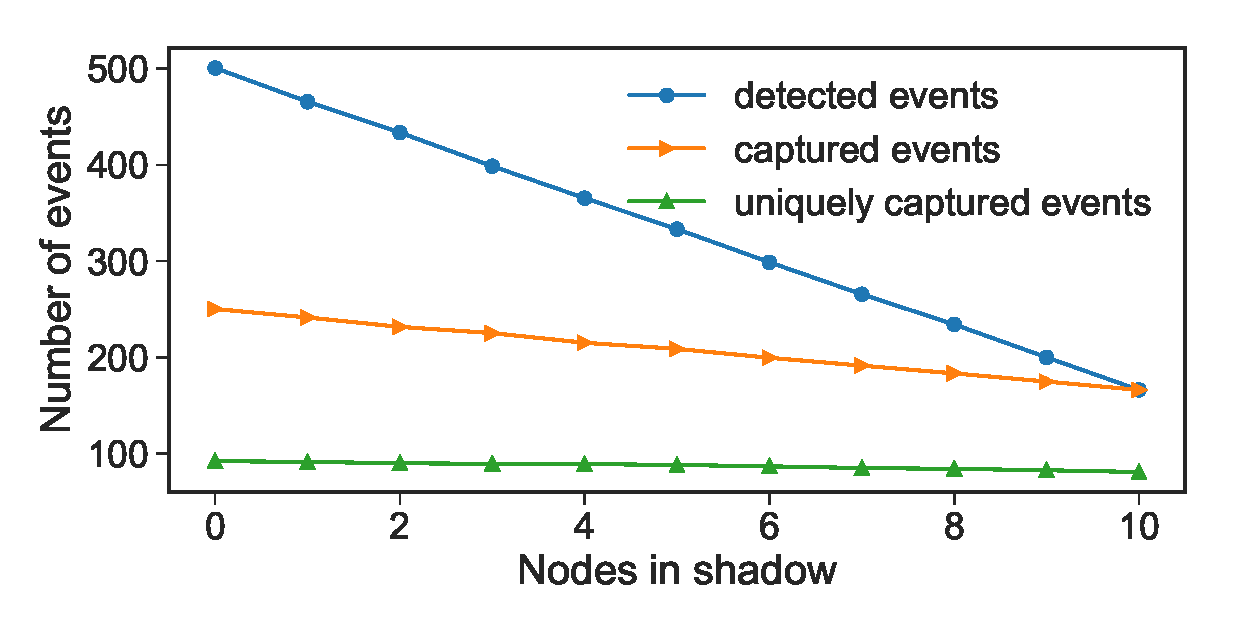
\includegraphics[width=\textwidth]{figures/different_energy_intensity}
		\caption{Simulated results showing how the number of captured events is affected when shadow is covering a \cis. Detected events are \#times events trigger nodes. Captured events are \#times nodes processed events. We used a redundent factor of 2.5 (see (\ref{eq:randFactor}))}.
		\label{fig:sim:differentEnergyIntensity}
	\end{subfigure}
	\vspace{-0.3cm}
	\caption{The effect of non-uniform energy distribution.}
	\label{fig:pwrCycleVSEnergyIntensity}
\end{figure}

\paragraph{Different energy harvesting rates}
It can happen that some of the nodes of a \cis are in the shadow while the rest is under direct sunlight (e.g., when curtains are being opened). 
As a consequence, nodes' power cycles will be significantly different (Figure~\ref{fig:fig:differentEnergyIntensity} shows the on-times, off-times, and power cycles when the ambient energy ranges from 400 to 1400\,lux). Therefore, nodes will not be able to accurately estimate the collective availability of the system. 
%
The inaccurate estimation is most significant when half of the nodes are in shadow. 
However, even during this worst case condition, a \cis availability is not dramatically effected (Figure~\ref{fig:sim:differentEnergyIntensity}). 
This because half of the nodes will overestimate the availability of the system while the other half underestimate the \cis's availability.
During this simulation the power cycles, on-time, and off-time of the nodes are 10, 5, and 5 unit of time when they are under sunlight and 24, 4, and 20 when they are in shadow. 
The length of the simulated experiment is 1000 unit of time.


% Taking into consideration that energy density vary overtime (e.g., the shadow of a curtain moves as the relative position of the curtain to the sun changes), an averaging technique might mitigate the negative effect of non-uniform distribution of ambient energy. However, we believe that these corner cases deserve a deeper and more extended study which is beyond the scope of this work.

\paragraph{Using machine learning algorithms to improve intermittent sensing}
In the future we plan to dive deeper in studying partially captured data. 
Intermittent sensors may partially capture events. Classical recognition 
algorithms face difficulties dealing with partially captured data. 
Therefore, we want to investigate \emph{how much machine learning algorithms 
can improve the sensing quality of intermittent sensing?} 
% \todo{MAC for backscattering and favorable energy conditions}




\section{Conclusion and Future Work}
Energy-harvesting battery-less sensors can operate very long because their power source is unlimited. 
However, ambient power is weak and volatile; therefore, these sensors operate intermittently.
The intermittent availability compromises their value as they have a high probability of missing events. 
This paper addresses the \emph{availability} problem of intermittent sensors. 
%
It presents the \textit{\fullcis} (\cis), which is the abstraction of a group of intermittently-powered sensors.
A \cis is able to approach continuous sensing by taking advantage of the embedded randomization in the powering subsystem of intermittent sensors.
The resulting differences in the sensor nodes' power cycles make the nodes' on-times uniformly distrusted. 
Therefore, the number of a \cis nodes can be seen as a design parameter to achieve a targeted collective availability. 
% Therefore, adding more nodes to a \cis increases its expected availability. 
We have modeled the availability of a \cis and its effective availability: the availability that leads to successful event capturing. 
Further, we showed the accuracy of these models by validating them against data collected on real hardware and with different ambient energy sources (i.e., sunlight, artificial light, and RF). 
%
Furthermore, we showed how the variation in nodes' power consumption and harvesting rate and the arrival of external events can compromise the \cis's availability (nodes employing sleeping mode to increase the chance of successfully capturing an event, synchronize their power cycles on the first incoming event, in a burst, and miss the subsequent ones. The probability of this unwanted synchronization increases when ambient energy rises beyond the design point.  
% It taking advantage of the embedded randomization in the powering subsystem of energy-harvesting battery-less sensors to distribute
% the on-times of a group of intermittent sensors uniformly in time 
% We presented the \textit{\fullcis} (\cis), an intermittently powered ``sensor'' that senses continuously! \cis is built around the observation that multiple intermittent nodes distribute themselves uniformly in time. This observation enables us to accurately model, and validate on real hardware, the \cis availability---the collective on-time of its intermittent nodes. 
% An important finding is that favorable energy conditions may cause sleeping intermittent nodes to synchronize their power cycles on the arrival of the first event. Consequently, they react to the same event, start recharging at the same time, and missing the next event. 
% 
To counter this unwanted behavior, we designed an algorithm to estimate the number of active neighbors and respond proportionally to an event. 
We developed a prototype of the \cis, an 8-nodes \fullCIM (\cim). 
Using this prototype, we showed that the \fullcis is able to distribute bursts of events on its nodes "evenly" and capture the entire burst with above 85\% detection accuracy.
 

Intermittent sensors will partially capture events. Classical algorithms for recognizing and classifying these events might face difficulties  dealing with partially captured data. Thus, follow-up work can investigate \emph{how much machine learning algorithms can improve the sensing quality of intermittent sensing?} 
% Additionally, the command recognition rate could further be improved by using an estimation of the energy left in the energy buffer, to start recharging early. This will prevent a detection when there is not enough harvested energy to record for a long enough time, letting a node recharge earlier and coming back with sufficient energy.


% \noindent\textbf{Speech Recognition on Intermittent Devices} In this paper, we have shown the feasibility of speech recognition on intermittent power. We also demonstrated the possibility of recognizing burst of events (in our case four words). However, the type of speech we targeted is the simplest, isolated words. Next, we may attempt recognizing a more complicated type of speech and for a larger number of words than the number chosen for this study.




\section{Acknowledgements}
We like to thank Stephan Wong for his contributions in the early stages of this
work, and the anonymous referees for their comments helping us to polish the
paper to perfection.



\bibliographystyle{ACM-Reference-Format}
\bibliography{references}

\end{document}
